\documentclass[runningheads]{paper}

\usepackage{hyperref}   % hyperlinks
\usepackage{graphicx}
\usepackage{algorithm}
\usepackage[noend]{algpseudocode}
\usepackage{multirow}
\usepackage{longtable}
\usepackage{float}
\usepackage{array}

% Used for displaying a sample figure. If possible, figure files should
% be included in EPS format.
%
% If you use the hyperref package, please uncomment the following line
% to display URLs in blue roman font according to Springer's eBook style:
% \renewcommand\UrlFont{\color{blue}\rmfamily}

% ------------------------------------------------------------------------------

\begin{document}
%
\title{Exploring the Utility of Machine Learning Across Varied Data Formats}
%
\author{Cărămidă Iustina-Andreea - 332CA}
%
\institute{Faculty of Automatic Control and Computer Science \\
University Politehnica of Bucharest \\
\email{iustina.caramida@stud.acs.upb.ro}
}
%
\maketitle              % typeset the header of the contribution
%
\begin{abstract}
    This study investigates the applicability of machine learning techniques on 
    diverse datasets. We explore the effectiveness of two algorithms, Linear 
    Regression and Multi-Layered Perceptron (MLP), on predicting both health 
    outcomes and financial well-being. Specifically, we utilize a stroke 
    prediction dataset to assess the model's ability to identify individuals at 
    risk of stroke. Additionally, we employ a salary prediction dataset to 
    evaluate the model's capacity to classify individuals earning above a 
    specific income threshold (e.g., \$50,000 per year). Through comparative 
    analysis, this research aims to elucidate the strengths and limitations of 
    each algorithm when applied to these contrasting data types, offering 
    insights into their suitability for various prediction tasks. Furthermore, 
    we present a framework for data analysis, outlining essential steps for data
    cleaning, exploration, and preparation, which can be applied to enhance the 
    effectiveness of machine learning models across diverse datasets.

\keywords{\textit{Machine Learning \and Heterogeneous Data \and Comparative Analysis \and
Prediction Modeling \and Data Analysis Techniques \and Stroke Prediction \and
Salary Prediction \and Linear Regression \and Multi-Layered Perceptron \and 
DataPreprocessing} }

\end{abstract}
% ------------------------------------------------------------------------------
\section{Introduction}

\subsection{Motivation: The Power and Nuance of Machine Learning Data}
Machine learning (ML) has become a cornerstone of progress in numerous 
disciplines. Its ability to extract valuable insights from vast and complex 
datasets has fueled breakthroughs in healthcare, finance, and social sciences. 
However, the effectiveness of ML models is not a one-size-fits-all proposition. 
Different data types possess unique characteristics, and understanding these 
nuances is essential for selecting the most appropriate ML algorithms. Data can 
be structured (organized in tables) or unstructured (text, images), numerical 
or categorical, and may exhibit linear or non-linear relationships between 
features.  Choosing the right algorithm depends heavily on these factors. This 
research delves into this crucial aspect of ML application by exploring the 
performance of two distinct algorithms on contrasting datasets.

\subsection{Research Focus: Delving into Stroke Prediction and Salary Prediction}
This study focuses on the application of ML techniques to two contrasting 
datasets: stroke prediction and salary prediction. Stroke, a leading cause of 
disability and death globally, poses a significant public health burden. Stroke 
prediction models aim to identify individuals at high risk of experiencing a 
stroke, allowing for preventive measures and early intervention. These models 
typically analyze factors such as age, blood pressure, cholesterol levels, and 
smoking history.

Conversely, salary prediction models attempt to classify individuals based on 
income thresholds. This information can offer valuable insights into economic 
trends, such as income inequality, and inform policy decisions. Salary 
prediction models might analyze factors like education level, work experience, 
and industry sector. By investigating these two distinct datasets, this research 
aims to gain a broader understanding of how ML algorithms perform on different 
data types with varying underlying structures and complexities.

\subsection{Methodology: Unveiling the Algorithms - Linear Regression and Multi-Layered Perceptron}
To investigate the performance on these contrasting datasets, this study employs 
two prominent ML algorithms: Linear Regression and Multi-Layered Perceptron (MLP). 

Linear Regression is a well\-established technique known for its interpretability
and efficiency in uncovering linear relationships between features (data points) 
and target variables (what we want to predict). This makes it a valuable tool 
for understanding the underlying factors influencing a particular outcome, such 
as the relationship between blood pressure and stroke risk. However, its strength 
lies in capturing linear relationships. If the underlying relationships in the 
data are more complex and non-linear, then Linear Regression might not be as 
effective.

On the other hand, Multi-Layered Perceptrons (MLPs) are a type of artificial 
neural network capable of learning complex, non-linear patterns within data. 
Unlike Linear Regression, MLPs are not limited by linearity and can potentially 
capture more intricate relationships between features and target variables. This 
capability makes them particularly suitable for datasets with complex underlying 
structures, such as the factors influencing an individual's salary, which might 
involve a combination of education, experience, industry, and other factors 
interacting in non-linear ways.

\subsection{Research Objectives: Evaluating Algorithms, Unveiling Strengths and Weaknesses}
By comparatively analyzing the performance of Linear Regression and MLP on 
stroke and salary prediction tasks, this research seeks to achieve several key 
objectives:

\subsubsection{Evaluate the Suitability of Algorithms for Diverse Data Types:}
This involves assessing the effectiveness of each algorithm in capturing the 
underlying relationships within the stroke prediction and salary prediction 
datasets. We will determine which algorithm performs better on each dataset, 
offering insights into their suitability for different data types, such as 
linear datasets (blood pressure and stroke risk) versus potentially non-linear 
datasets (factors influencing salary).

\subsubsection{Gain Insights into Algorithmic Strengths and Weaknesses:}
By analyzing the comparative performance, we aim to highlight the scenarios where
each algorithm excels and identify areas where one might outperform the other. 
This will provide valuable guidance for researchers and practitioners in 
selecting the most appropriate algorithm for their specific prediction tasks. 
For instance, if interpretability is crucial (e.g., understanding the factors 
influencing stroke risk), Linear Regression might be preferred. If the data is 
likely to have complex, non-linear relationships, then an MLP might be a better 
choice.

\subsubsection{Demonstrate Best Practices for Data Analysis in ML Applications:}
Effective data analysis is crucial for building robust ML models. This research 
will showcase essential steps for data cleaning, exploration, and preparation, 
emphasizing their importance in enhancing model performance across diverse 
datasets. These steps may include handling missing values, identifying outliers, 
and feature engineering (creating new features from existing data) to improve 
the model's ability to learn from the data.

\subsection{Expected Contribution: Advancing the Application of ML on Heterogeneous Data}
Through this exploration, the research aims to contribute valuable knowledge to 
the field of machine learning, particularly the application of ML on 
heterogeneous datasets.  The findings can guide researchers and practitioners 
in selecting appropriate algorithms for their specific prediction tasks and 
data types.  Furthermore, by demonstrating best practices for data analysis, 
this research can contribute to the development of more robust and reliable ML 
models across diverse application domains. This can lead to advancements in 
areas like healthcare (improved stroke prediction for preventive measures) and 
economics (better understanding of factors influencing income inequality).  
Ultimately, the research aims to contribute to the responsible and effective use 
of ML for tackling complex problems across various fields.
% ------------------------------------------------------------------------------
\section{Exploratory Data Analysis}

\subsection{Datasets attributes description}
The initial and crucial step in developing any machine learning algorithm 
involves a thorough understanding of the data it will be trained on. This 
understanding is achieved through a comprehensive analysis of the datasets' 
characteristics. In this vein, the following sub sections will delve into the 
specific attributes of the two datasets employed in this study: stroke 
prediction and salary prediction.

A detailed description of each salary prediction attribute is provided in Table
\ref{tab:salary_attributes_description} and of each stroke  prediction attribute
in Table \ref{tab:stroke_attributes_description}.

\begin{center}
    \begin{longtable}{ |>{\centering\arraybackslash}p{3cm}||>{\centering\arraybackslash}p{2cm}|>{\centering\arraybackslash}p{6cm}| }
        \hline
        \multicolumn{3}{|c|}{List of all attributes in the Salary Prediction dataset} \\
        \hline
        Attribute name & Type & Details \\
        \hline
        fnl & numeric & Socio-economic characteristic of the population from which the individual comes \\
        \hline
        hpw & numeric & Number of work hours per week \\
        \hline
        relation & categorical & The type of relationship in which the individual is involved \\
        \hline
        gain & numeric & Capital gain \\
        \hline
        country & categorical & Country of origin \\
        \hline
        job & categorical & The individual's job \\
        \hline
        edu\_int & numeric & Number of years of study \\
        \hline
        years & numeric & Age of the individual \\
        \hline
        loss & numeric & Loss of capital \\
        \hline
        work\_type & categorical & The job's type \\
        \hline
        partner & categorical & The type of partner the individual has \\
        \hline
        edu & categorical & The individual's type of education \\
        \hline
        gender & categorical & Individual's gender \\
        \hline
        race & categorical & Individual's race \\
        \hline
        prod & numeric & Capital production \\
        \hline
        gtype & categorical & Type of employment contract \\
        \hline
        money & categorical & Whether the individual earns more than \$50,000 per year \\
        \hline
        \caption{Salary Prediction Attributes}
        \label{tab:salary_attributes_description}
   \end{longtable}
\end{center}

\begin{center}
    \begin{longtable}{ |>{\centering\arraybackslash}m{3.5cm}||>{\centering\arraybackslash}m{2cm}|>{\centering\arraybackslash}m{3.5cm}|>{\centering\arraybackslash}m{2.5cm}| }
        \hline
        \multicolumn{4}{|c|}{List of all attributes in the Stroke Prediction dataset} \\
        \hline
        Attribute name & Type & Details & Possible values \\
        \hline
        mean\_blood\_sugar\_ level & numeric & The average value of blood glucose throughout the duration observation of the subject & \\
        \hline
        cardiovascular\_issues & categorical & Whether or not the subject has a medical history cardiovascular & 0, 1 \\
        \hline
        job\_category & categorical & The field in which the person works & child, entrepreneurial, N\_work\_history, private\_sector, public\_sector \\
        \hline
        body\_mass\_indicator & numeric & Body mass index, which indicates if the person is underweight, within limits normal, overweight or obese & \\
        \hline
        sex & categorical & The gender of the person & F, M\\
        \hline
        tobacco\_usage & categorical & Current or past smoker indicator &  ex-smoker, smoker, non-smoker\\
        \hline
        high\_blood\_pressure & categorical & Binary attribute indicating whether a person suffer from high blood pressure or not & 0, 1 \\
        \hline
        married & categorical & Binary attribute indicating whether the person a ever been married & Y, N \\
        \hline
        living\_area & categorical & The type of area where he lived most of his life & City, Countryside \\
        \hline
        years\_old & numeric & The person's age in years & \\
        \hline
        chaotic\_sleep & categorical & Binary attribute for a sleep program irregular & 0, 1 \\
        \hline
        analysis\_results & numeric & The results of medical analyzes of the person, which may include various measurements and indicators relevant to her health & \\
        \hline
        biological\_age\_index & numeric & An index that estimates the biological age of a person based on different factors such as lifestyle, health status, measured in an unknown unit & \\
        \hline
        cerebrovascular\_ accident & categorical & Binary indicator indicating whether the person a had a stroke or not & 0, 1 \\
        \hline
        \caption{Stroke Prediction Attributes}
        \label{tab:stroke_attributes_description}
   \end{longtable}
\end{center}

\subsection{Exploration of Attribute Types and Value Ranges}
Prior to applying a machine learning model to a dataset, a crucial step involves
in identifying the types of attributes (features) present and their corresponding
values ranges. This anaysis is essential for selecting appropriate algorithms 
and ensuring optimal model performance. In the following pharagraphs we will
describe three primary attribute types.
\begin{itemize}
    \item \textit{Continuous Numeric Attributes:}
    These attributes possess numerical values that can theoretically take on any 
    value within a specific range. Examples might include: age, weight, temperature etc.
    \item \textit{Discrete Nominal Attributes:}
    These attributes represent categorical data with distinct, non-ordered values. 
    Examples include days of the week (Monday, Tuesday, etc.) or types of diseases 
    (cancer, diabetes, etc.).
    \item \textit{Ordinal Attributes:}
    These attributes represent categorical data with values that exhibit an inherent 
    order. However, the difference between consecutive values may not be interpretable 
    in terms of a consistent unit.  Examples include customer satisfaction ratings 
    (1-star, 2-star, etc.) or movie ratings (G, PG, PG-13, etc.). In ordinal 
    attributes, the numerical value itself might not be as important as the relative 
    order it represents.
\end{itemize}

Using the \textit{analysis\_attributes.py} script, we can identify the 
Continuous Numeric Attributes and Discrete Nominal Attributes in the  
datasets. The script will output statistics that can be showed in Tables 
\ref{tab:continuous_numeric_attributes_salary} and 
\ref{tab:continuous_numeric_attributes_stroke} for numeric attributes and
Table \ref{tab:discrete_nominal_attributes_salary} and 
\ref{tab:discrete_nominal_attributes_stroke} for discrete attributes.

Moreover, the total number of items in the full dataset is 9999 for the Salary
Prediction dataset and 5110 for the Stroke Prediction dataset.


\begin{center}
    \begin{longtable}{ |>{\centering\arraybackslash}m{0.95cm}||>{\centering\arraybackslash}m{1.75cm}|>{\centering\arraybackslash}m{1.75cm}|>{\centering\arraybackslash}m{1.75cm}|>{\centering\arraybackslash}m{1.75cm}|>{\centering\arraybackslash}m{1.75cm}|>{\centering\arraybackslash}m{1.75cm}|>{\centering\arraybackslash}m{1.75cm} |}
        \hline
        \multicolumn{8}{|c|}{List of all Continuous Numeric Attributes in the Salary Prediction dataset} \\
        \hline
         & fnl & hpw & gain & edu\_int & years & loss & prod \\
        \hline\hline
        count & 9.999000e +03 & 9199.00000 & 9999.00000 & 9999.00000 & 9999.00000 & 9999.00000 & 9999.00000 \\
        \hline
        mean &  1.903529e +05 & 40.416241 & 979.853385 & 14.262026 & 38.646865 & 84.111411 & 2014.9275 93 \\
        \hline
        std & 1.060709e +05 & 12.517356 & 7003.7953 82 & 24.770835 & 13.745101 & 3394.0354 84 & 14007.6044 96 \\
        \hline
        min & 1.921400e +04 & 1.000000 & 0.000000 & 1.000000 & 17.000000 & 0.000000 & -28.000000 \\
        \hline
        25\% & 1.182825e +05 & 40.000000 & 0.000000 & 9.000000 & 28.000000 & 0.000000 & 42.000000 \\
        \hline
        50\% & 1.784720e +05 & 40.000000 & 0.000000 & 10.000000 & 37.000000 & 0.000000 & 57.000000 \\
        \hline
        75\% & 2.373110e +05 & 45.000000 & 0.000000 & 13.000000 & 48.000000 & 0.000000 & 77.000000 \\
        \hline
        max & 1.455435e +06 & 99.00000 & 99999.0000 & 206.000000 & 90.000000 & 3770.00000 & 200125.000 \\
        \hline
        \caption{Continuous Numeric Attributes in Salary Prediction Dataset}
        \label{tab:continuous_numeric_attributes_salary} \\
   \end{longtable}
\end{center}

\begin{center}
    \begin{longtable}{ |>{\centering\arraybackslash}m{0.95cm}||>{\centering\arraybackslash}m{2.45cm}|>{\centering\arraybackslash}m{2.45cm}|>{\centering\arraybackslash}m{2.45cm}|>{\centering\arraybackslash}m{2.45cm}|>{\centering\arraybackslash}m{2.45cm}| }
        \hline
        \multicolumn{6}{|c|}{List of all Continuous Numeric Attributes in the Stroke Prediction dataset} \\
        \hline
        & mean\_blood\_ sugar\_level & body\_mass\_ indicator & years\_old & analysis\_results & biological\_age\_ index \\
        \hline\hline
        count & 5110.000000 & 4909.000000 & 5110.000000 & 4599.000000 & 5110.000000 \\
        \hline
        mean & 106.147677 & 28.893237 & 46.568665 & 323.523446 & 134.784256 \\
        \hline
        std & 45.283560 & 7.854067 & 26.593912 & 101.577442 & 50.399352 \\
        \hline
        min & 55.120000 & 10.300000 & 0.080000 & 104.829714 & -15.109456 \\
        \hline
        25\% & 77.245000 & 23.500000 & 26.000000 & 254.646209 & 96.710581 \\
        \hline
        50\% & 91.885000 & 28.100000 & 47.000000 & 301.031628 & 136.374631 \\
        \hline
        75\% & 114.090000 & 33.100000 & 63.750000 & 362.822769 & 172.507322 \\
        \hline
        max & 271.740000 & 97.600000 & 134.000000 & 756.807975 & 266.986321 \\
        \hline
        \caption{Continuous Numeric Attributes in Stroke Prediction Dataset}
        \label{tab:continuous_numeric_attributes_stroke} \\
    \end{longtable}
\end{center}

An initial inspection of the data reveals that there are missing attributes in 
both the Salary Prediction and Stroke Prediction datasets. In the Salary Prediction 
datase the \textit{'hpw'} attribute is missing, while int the Stroke Prediction dataset
two attributes are missing: \textit{'body\_mass\_indicator'} and 
\textit{'analysis\_results'}.

To better understand the distribution of the continuous numeric attributes 
within the datasets, boxplots have been generated for each attribute. These 
visualizations are located in the \textit{'plots'} folder at the root of the 
project directory. The name of each boxplot starts with \textit{'box\_plot\_'}.

Boxplots are a standardized method for visually representing the distribution of
data.  They provide insights into several key characteristics of the data, 
including the median, quartiles, and outliers.

In the Figure \ref{fig:boxplot_example_salary} we can see a boxplot for the 
\textit{years} attribute in the Salary Prediction dataset. The box in the middle
of the plot contains the middle 50\% of the data, and the line in the middle
represents the median. The whiskers extend to the minimum and maximum values
within 1.5 times the interquartile range (the difference between the first and
third quartiles). Points outside this range are considered outliers.

Also, in Figure \ref{fig:boxplot_example_stroke} we can see a boxplot for the
\textit{body\_mass\_indicator} attribute in the Stroke Prediction dataset.
As described above, the boxplot provides a visual representation of the data's
distribution, highlighting key statistical measures such as the median, quartiles,
and potential outliers. These information is also presented in Tables
\ref{tab:continuous_numeric_attributes_salary} and
\ref{tab:continuous_numeric_attributes_stroke}. One of the main insights that
can be derived from the boxplot is the presence of outliers, which are data points
that lie significantly outside the range of the rest of the data. Outliers can
have a significant impact on the performance of machine learning models, and
identifying and handling them appropriately is an essential step in the data
preprocessing process.

\begin{figure}[H]
    \centering
    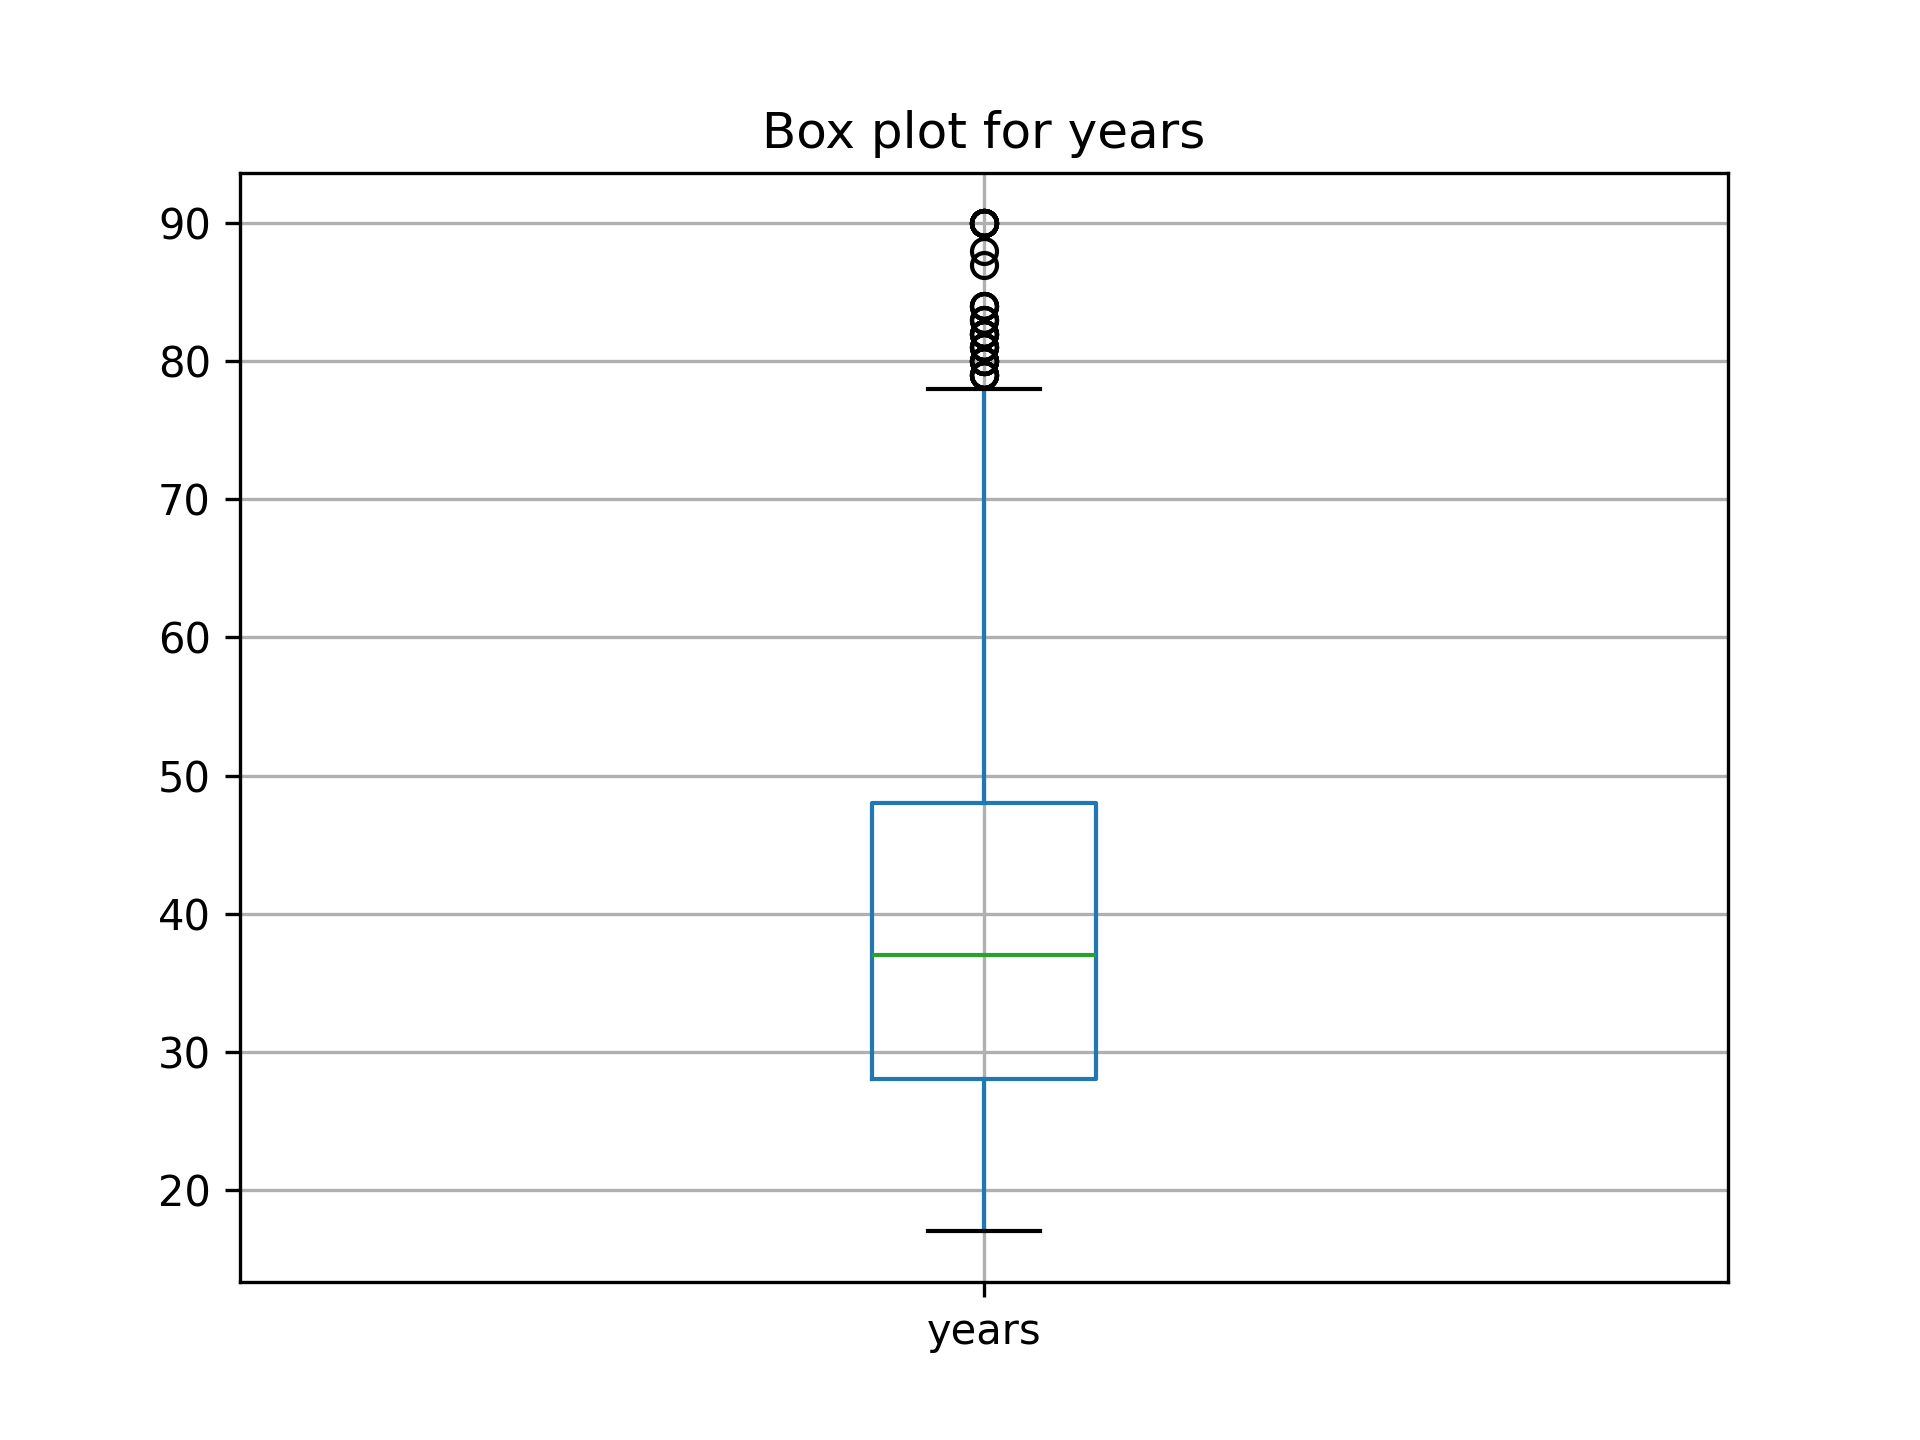
\includegraphics[width=0.8\textwidth]{../plots/box_plot_years_SalaryPrediction_full.png}
    \caption{Boxplot for the \textit{years} attribute in the Salary Prediction dataset}
    \label{fig:boxplot_example_salary}
\end{figure}

\begin{figure}[H]
    \centering
    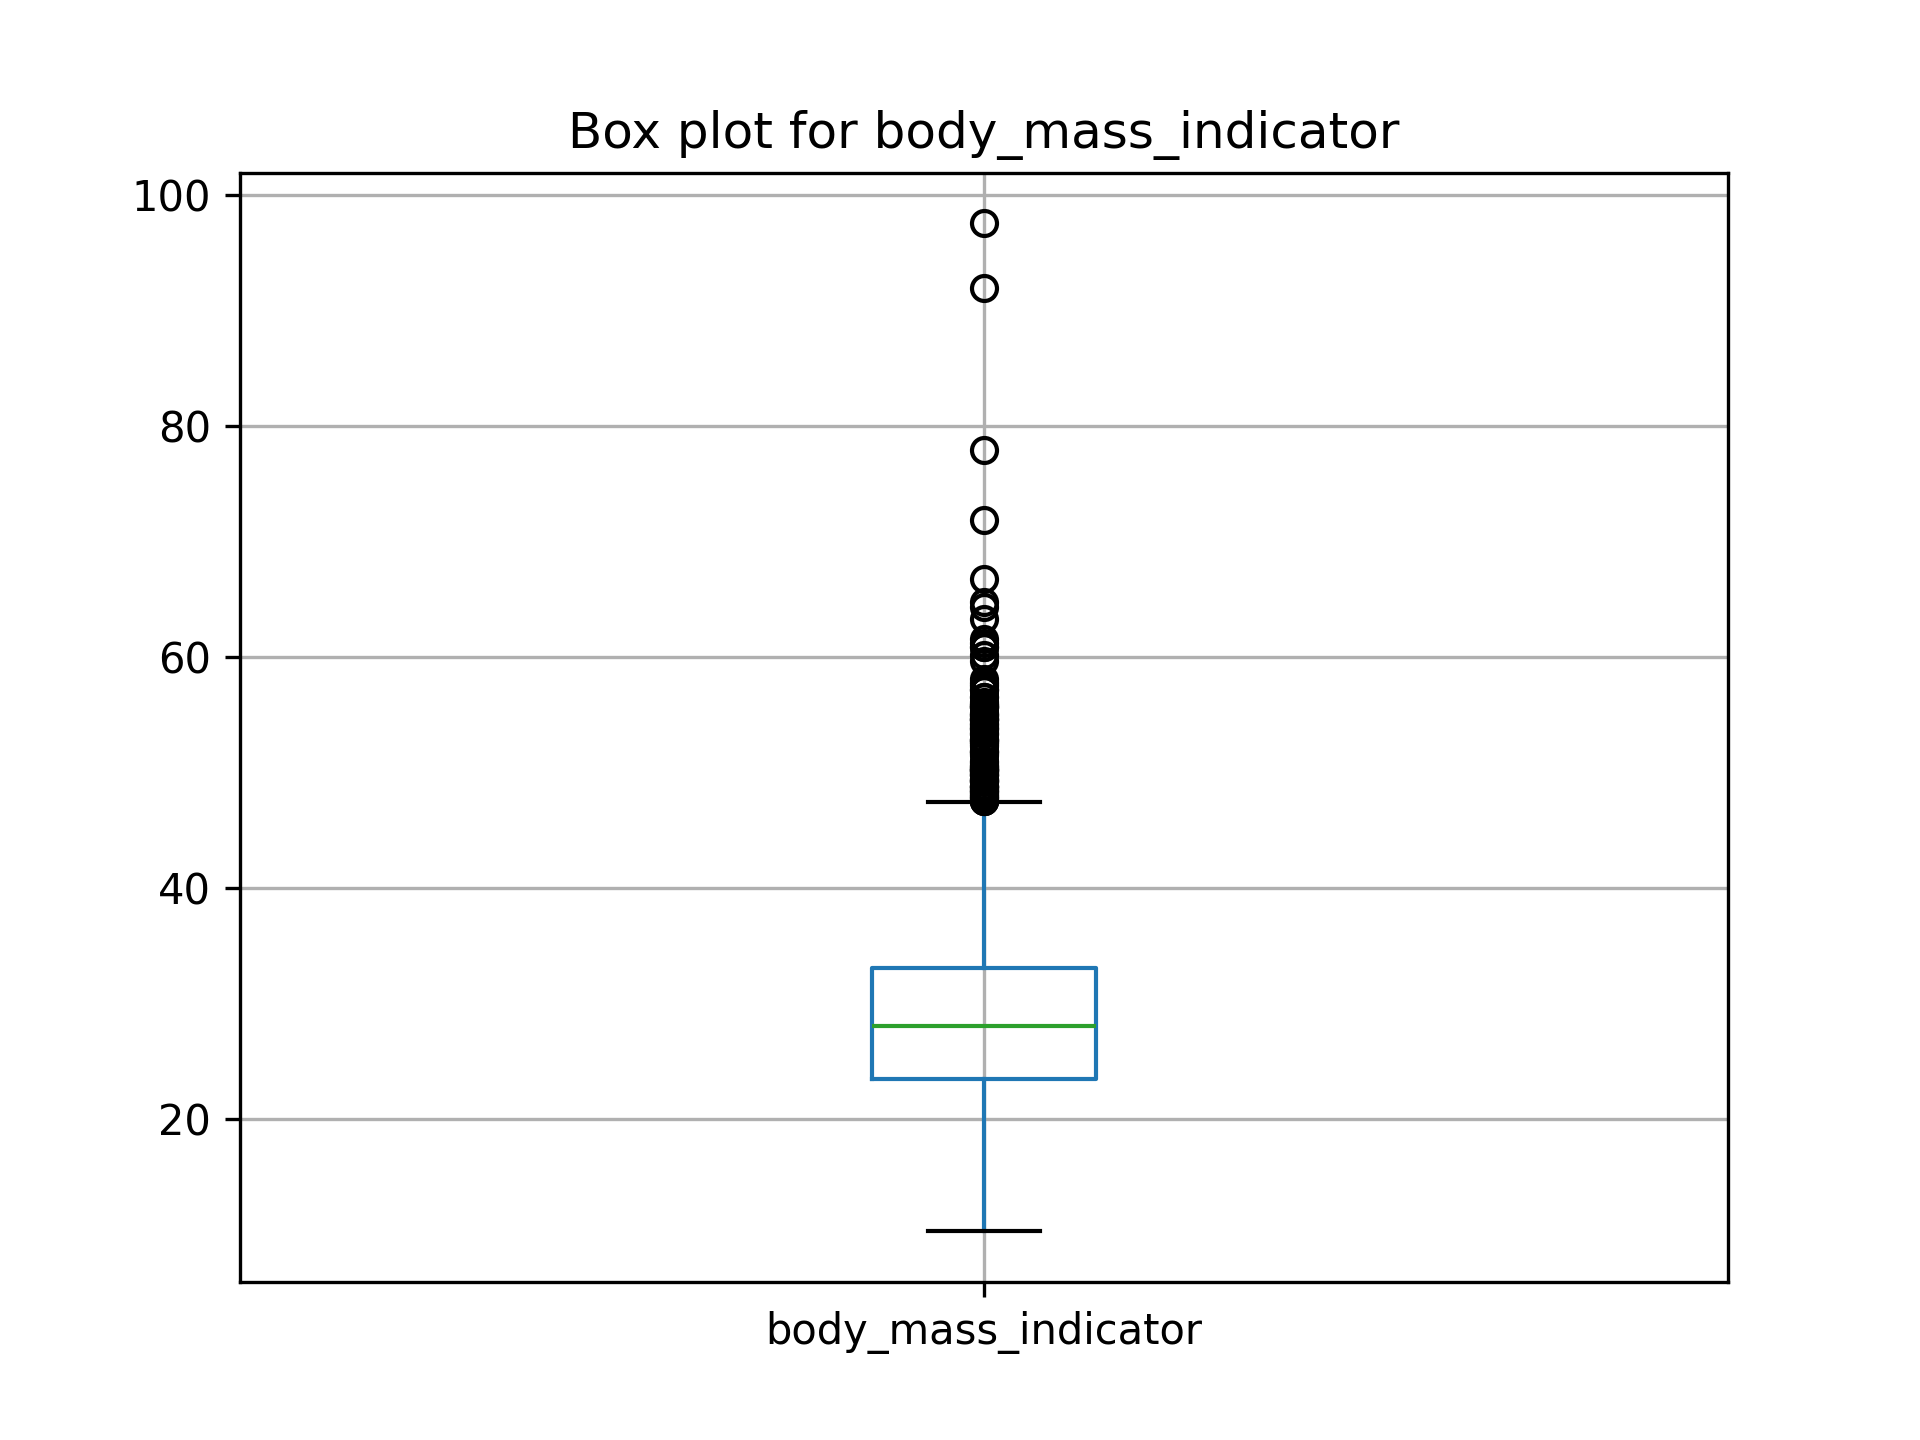
\includegraphics[width=0.8\textwidth]{../plots/box_plot_body_mass_indicator_AVC_full.png}
    \caption{Boxplot for the \textit{body\_mass\_indicator} attribute in the Stroke Prediction dataset}
    \label{fig:boxplot_example_stroke}
\end{figure}


\begin{center}
    \begin{longtable}{ |>{\centering\arraybackslash}m{5cm}||>{\centering\arraybackslash}m{3cm}|>{\centering\arraybackslash}m{3cm}|}
        \hline
        \multicolumn{3}{|c|}{List of all Discrete Nominal Attributes in the Salary Prediction dataset} \\
        \hline
        & Non-missing count & Unique values count \\
        \hline\hline
        relation & 9999 & 6 \\
        \hline
        country & 9999 & 41 \\
        \hline
        job & 9999 & 14 \\
        \hline
        work\_type & 9999 & 9 \\
        \hline
        partner & 9999 & 7 \\
        \hline
        edu & 9999 & 16 \\
        \hline
        gender & 9199 & 2 \\
        \hline
        race & 9999 & 5 \\
        \hline
        gtype & 9999 & 2 \\
        \hline
        money & 9999 & 2 \\
        \hline
        \caption{Discrete Nominal Attributes in Salary Prediction Dataset}
        \label{tab:discrete_nominal_attributes_salary} \\
    \end{longtable}
\end{center}

\begin{center}
    \begin{longtable}{ |>{\centering\arraybackslash}m{5cm}||>{\centering\arraybackslash}m{3cm}|>{\centering\arraybackslash}m{3cm}|}
        \hline
        \multicolumn{3}{|c|}{List of all Discrete Nominal Attributes in the Stroke Prediction dataset} \\
        \hline
        & Non-missing count & Unique values count \\
        \hline\hline
        cardiovascular\_issues & 5110 & 2 \\
        \hline
        job\_category & 5110 & 5 \\
        \hline
        sex & 5110 & 2 \\
        \hline
        tobacco\_usage & 5110 & 4 \\
        \hline
        high\_blood\_pressure & 5110 & 2 \\
        \hline
        married & 4599 &2 \\
        \hline
        living\_area & 5110 & 2 \\
        \hline
        chaotic\_sleep & 5110 & 2 \\
        \hline
        cerebrovascular\_accident & 5110 & 2 \\
        \hline

        \caption{Discrete Nominal Attributes in Stroke Prediction Dataset}
        \label{tab:discrete_nominal_attributes_stroke} \\
    \end{longtable}
\end{center}

From the Discret Nominal Attributes tables (Tables \ref{tab:discrete_nominal_attributes_salary} and \ref{tab:discrete_nominal_attributes_stroke})
we can see that each dataset contains
only one attribute with missing values. In the Salary Prediction dataset 
the \textit{gender} attribute is missing, while the Stroke Prediction dataset the
\textit{married} attribute is missing. Also, the number of unique values for each attribute
descibes the diversity of the data. For example, the \textit{country} attribute
in the Salary Prediction dataset has 41 unique values, indicating that the data
contains information from 41 different countries.

In the historigrams for the discrete nominal attributes, we can see the
distribution of the unique values for each attribute. These visualizations can
provide insights into the frequency of each category within the dataset, which
can be useful for understanding the data's composition and identifying potential
imbalances or biases. The histograms for the discrete nominal attributes are
located in the \textit{'plots'} folder at the root of the project directory.
The name of each histogram starts with \textit{'histogram\_'}.

\begin{figure}[H]
    \centering
    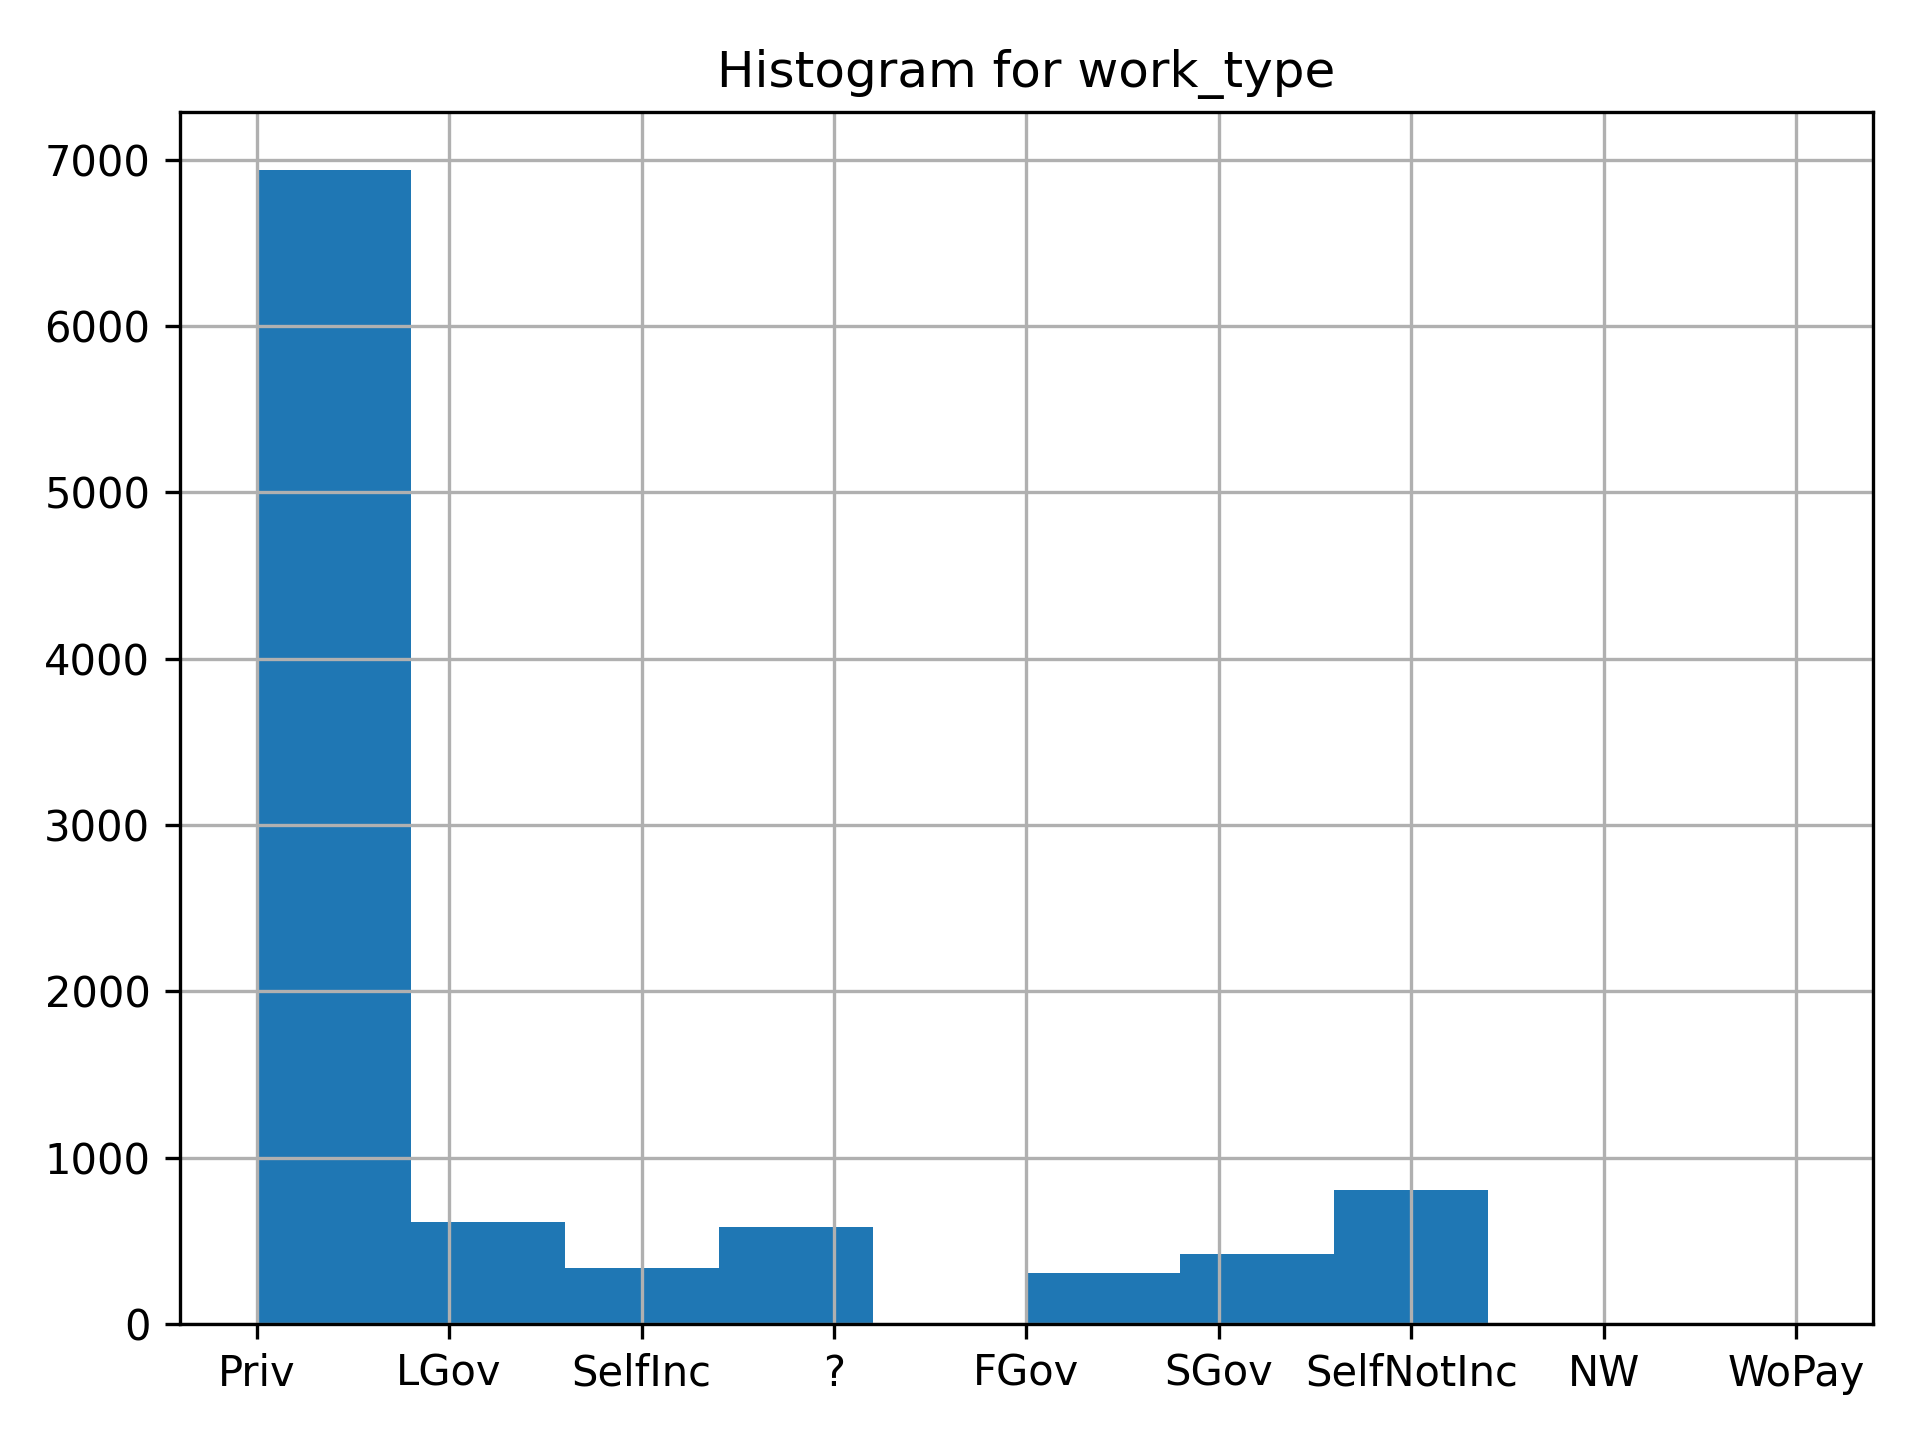
\includegraphics[width=0.8\textwidth]{../plots/histogram_work_type_SalaryPrediction_full.png}
    \caption{Histogram for the \textit{work\_type} attribute in the Salary Prediction dataset}
    \label{fig:histogram_example_salary}
\end{figure}

\begin{figure}[H]
    \centering
    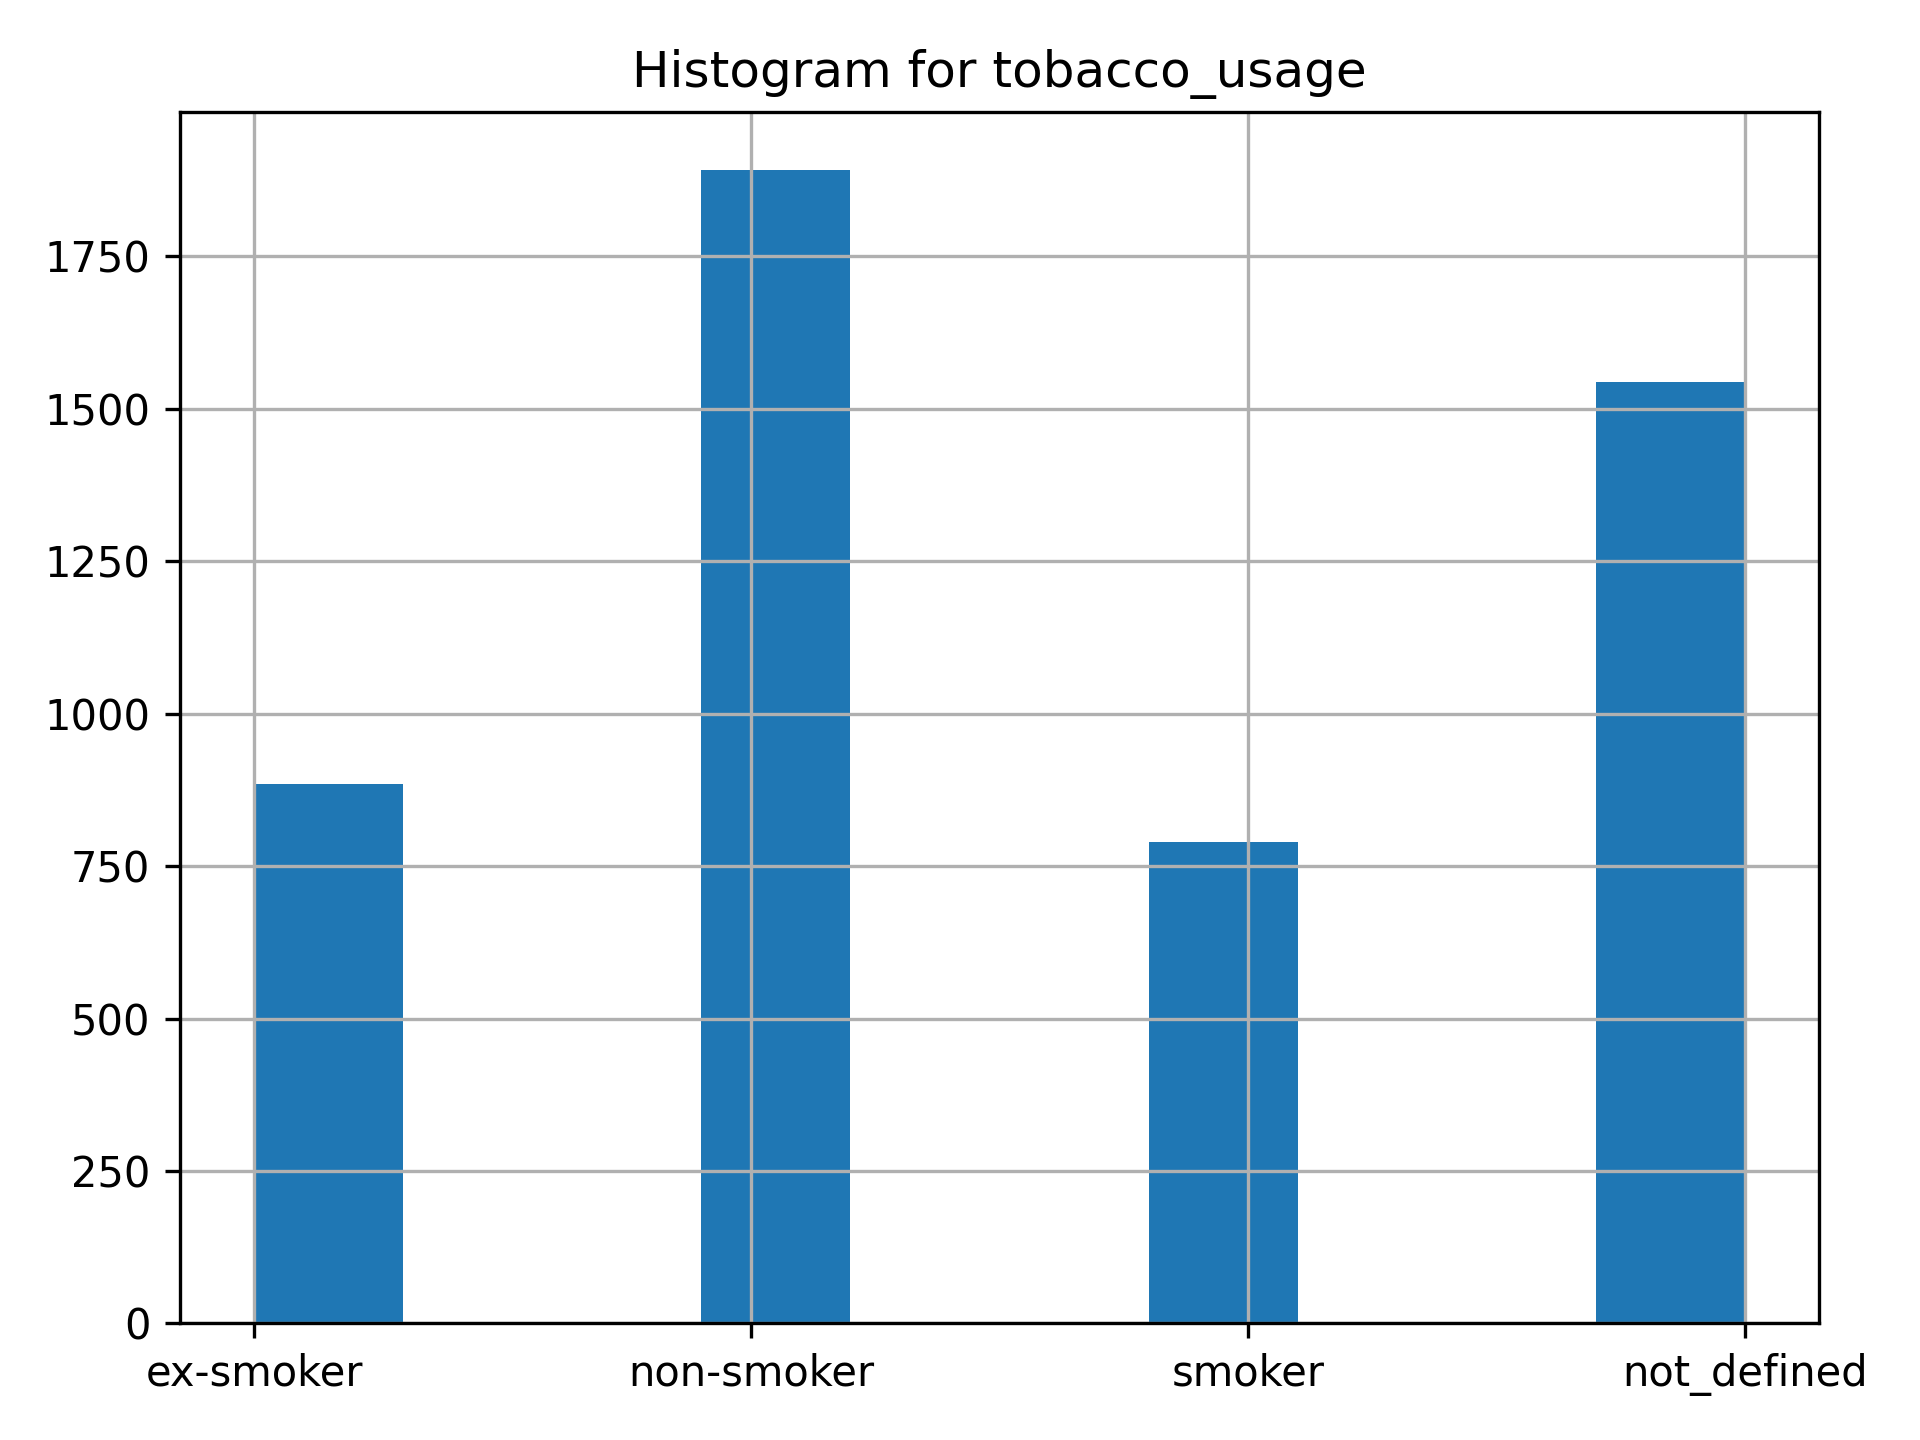
\includegraphics[width=0.8\textwidth]{../plots/histogram_tobacco_usage_AVC_full.png}
    \caption{Histogram for the \textit{tobacco\_usage} attribute in the Stroke Prediction dataset}
    \label{fig:histogram_example_stroke}
\end{figure}

In Figure \ref{fig:histogram_example_salary} we can see a histogram of the
\textit{work\_type} attribute in the Salary Prediction dataset. The dominance of
the 'Priv' category indicates a severe class imbalance. For classification tasks,
the model might predict Priv most of the time since it's the majority class, 
leading to a high overall accuracy but poor precision, recall, and F1 scores 
for minority classes.

Also, in Figure \ref{fig:histogram_example_stroke} we can see a histogram of the
\textit{tobacco\_usage} attribute in the Stroke Prediction dataset. The histogram 
shows that the majority of individuals are non-smokers, with a significant portion 
having undefined tobacco usage status. This imbalance and the presence of missing 
data need to be addressed appropriately.

\subsection{Investigation of Class Distribution}
In machine learning, it is common practice to split a dataset into two distinct
subsets: a training set and a test set. This division is crucial for ensuring 
 robustness and generalizability of the models developed using the data.

\begin{itemize}
    \item \textbf{Training Set:} The primary purpose of the training set is to 
    train the machine 
    learning model. The model learns from patterns and relationships within the data 
    to develop a predictive capability.
    \item \textbf{Test Set:} The test set, unseen by the model during training, 
    serves to evaluate the model's generalizability. By applying the trained 
    model to the test set, we can assess its performance on new, unseen data. 
    This helps prevent overfitting, where the model performs well on the 
    training data but fails to generalize to real-world scenarios.
\end{itemize}

Looking at how data is distributed is key. Imbalanced data, where some classes 
have far more examples than others, throws off classification tasks:
high accuracy can hide poor performance on rare classes; models struggle to 
learn patterns from underrepresented classes; inaccurate predictions, especially 
for the minority class.

By checking the distribution, we can address imbalance:
\begin{itemize}
    \item Balance the data: Oversample rare examples or undersample common ones.
    \item Cost-sensitive learning: Penalize the model more for mistakes on rare classes.
    \item Better metrics: Use precision, recall, and F1-score to get a clearer picture.
\end{itemize}

In Figures \ref{fig:distribution_salary} and \ref{fig:distribution_stroke} we can
see the distribution of each class in the datasets. The class distributions provide
insights into the balance of the data and can help guide the selection of appropriate
strategies for handling imbalanced classes. For example, in the Stroke Prediction
dataset, the \textit{cerebrovascular\_accident} class is highly imbalanced, with
a significantly higher number of negative instances compared to positive instances.
This imbalance can impact the model's ability to learn patterns from the minority
class and may require resampling techniques or cost-sensitive learning to address.
On the other hand, the Salary Prediction dataset exhibits a more balanced distribution
of the \textit{money} class, which may require less intervention to handle class
imbalance.

\begin{figure}[H]
    \centering
    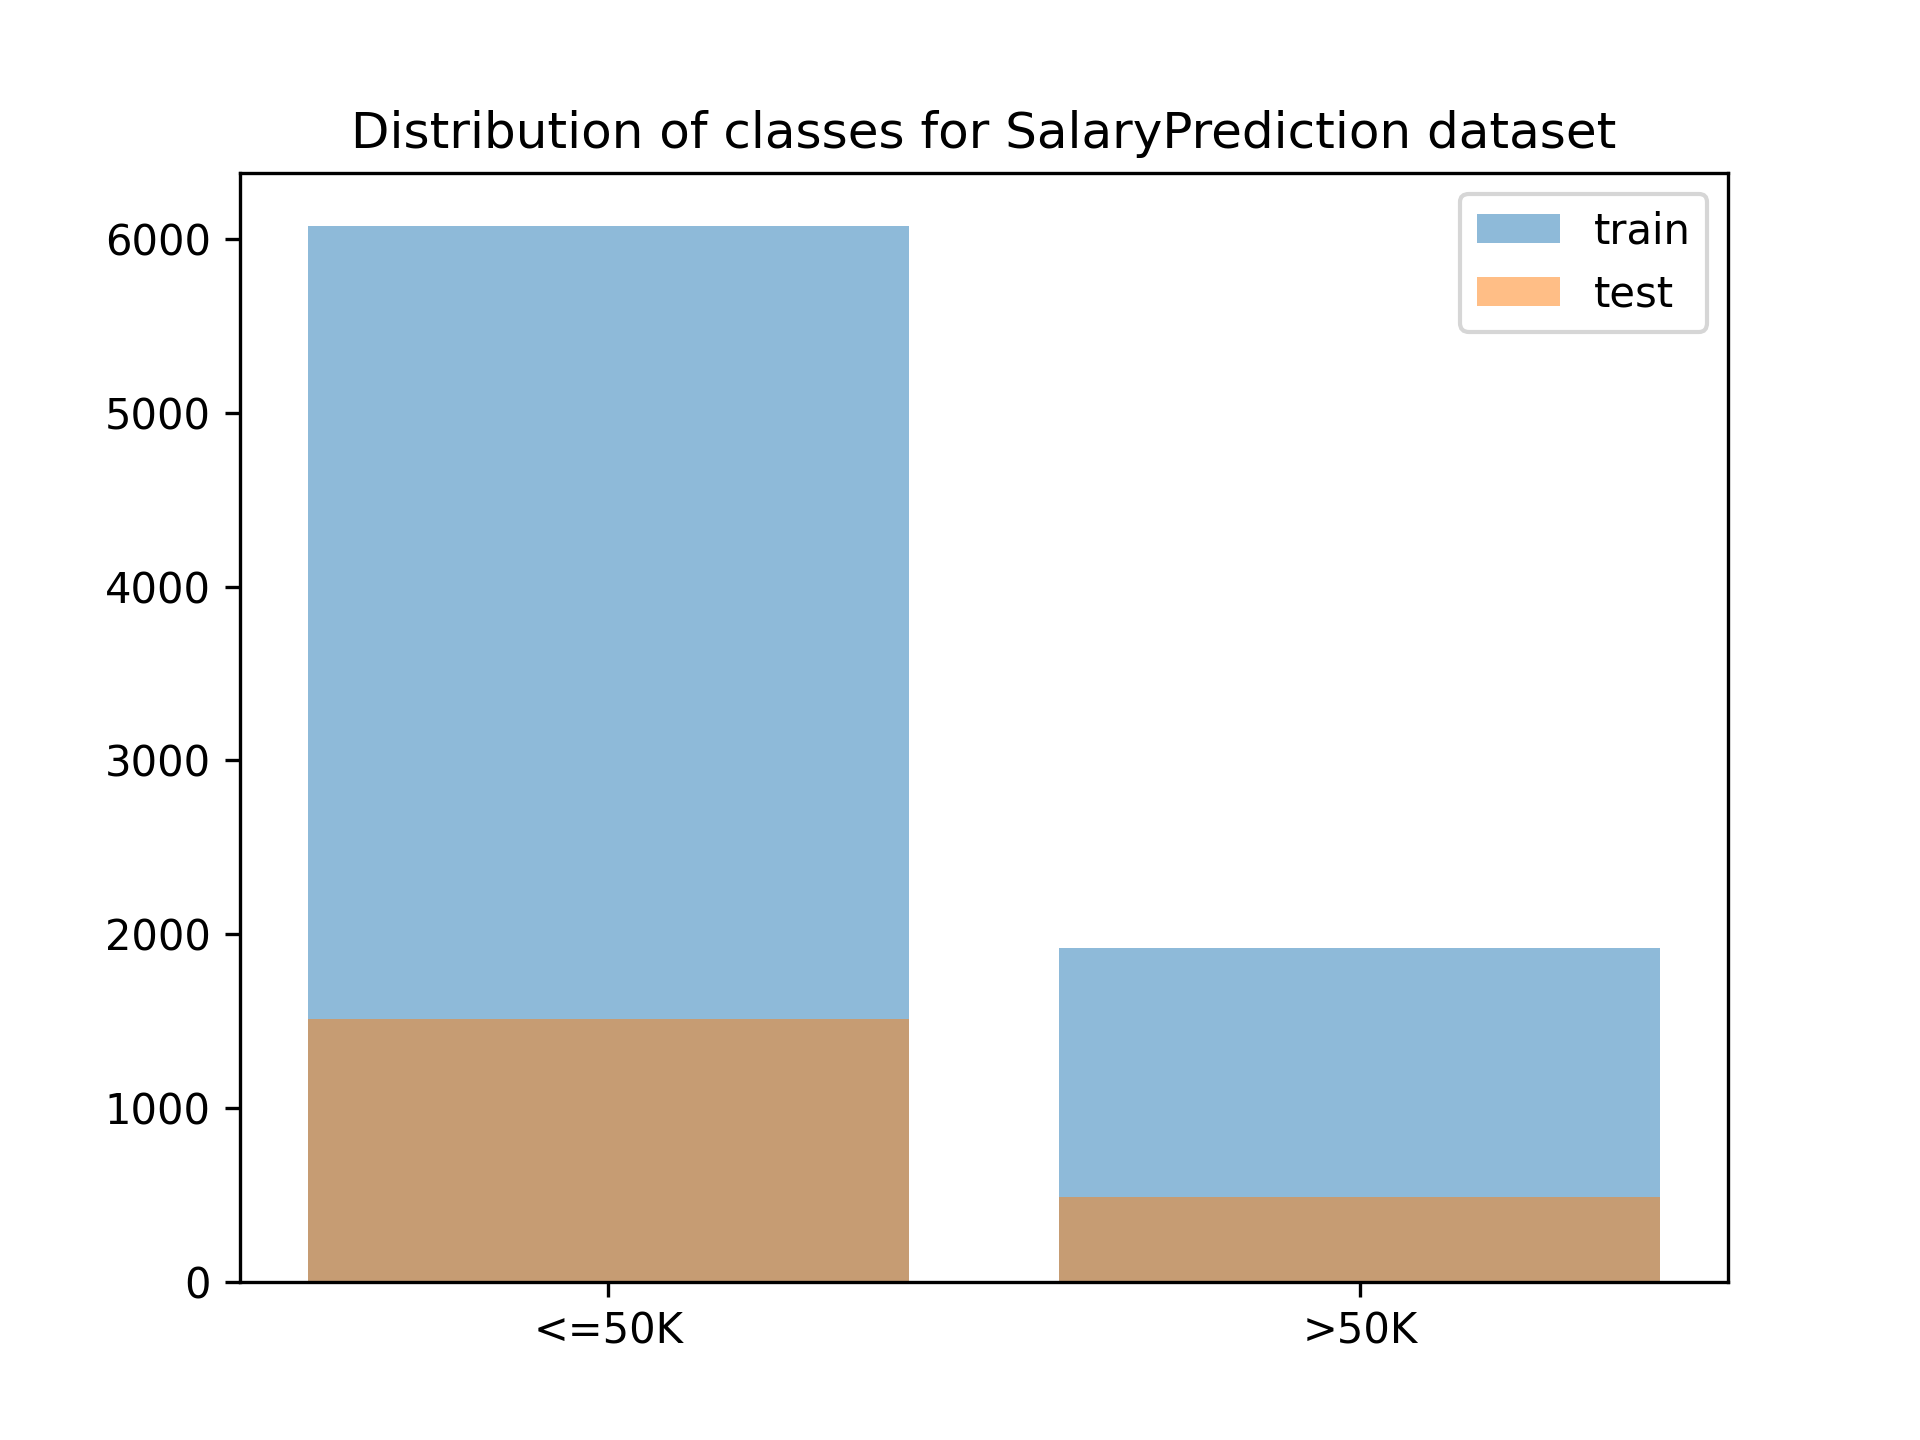
\includegraphics[width=0.8\textwidth]{../plots/distribution_SalaryPrediction.png}
    \caption{Distribution of the \textit{money} class in the Salary Prediction dataset}
    \label{fig:distribution_salary}
\end{figure}

\begin{figure}[H]
    \centering
    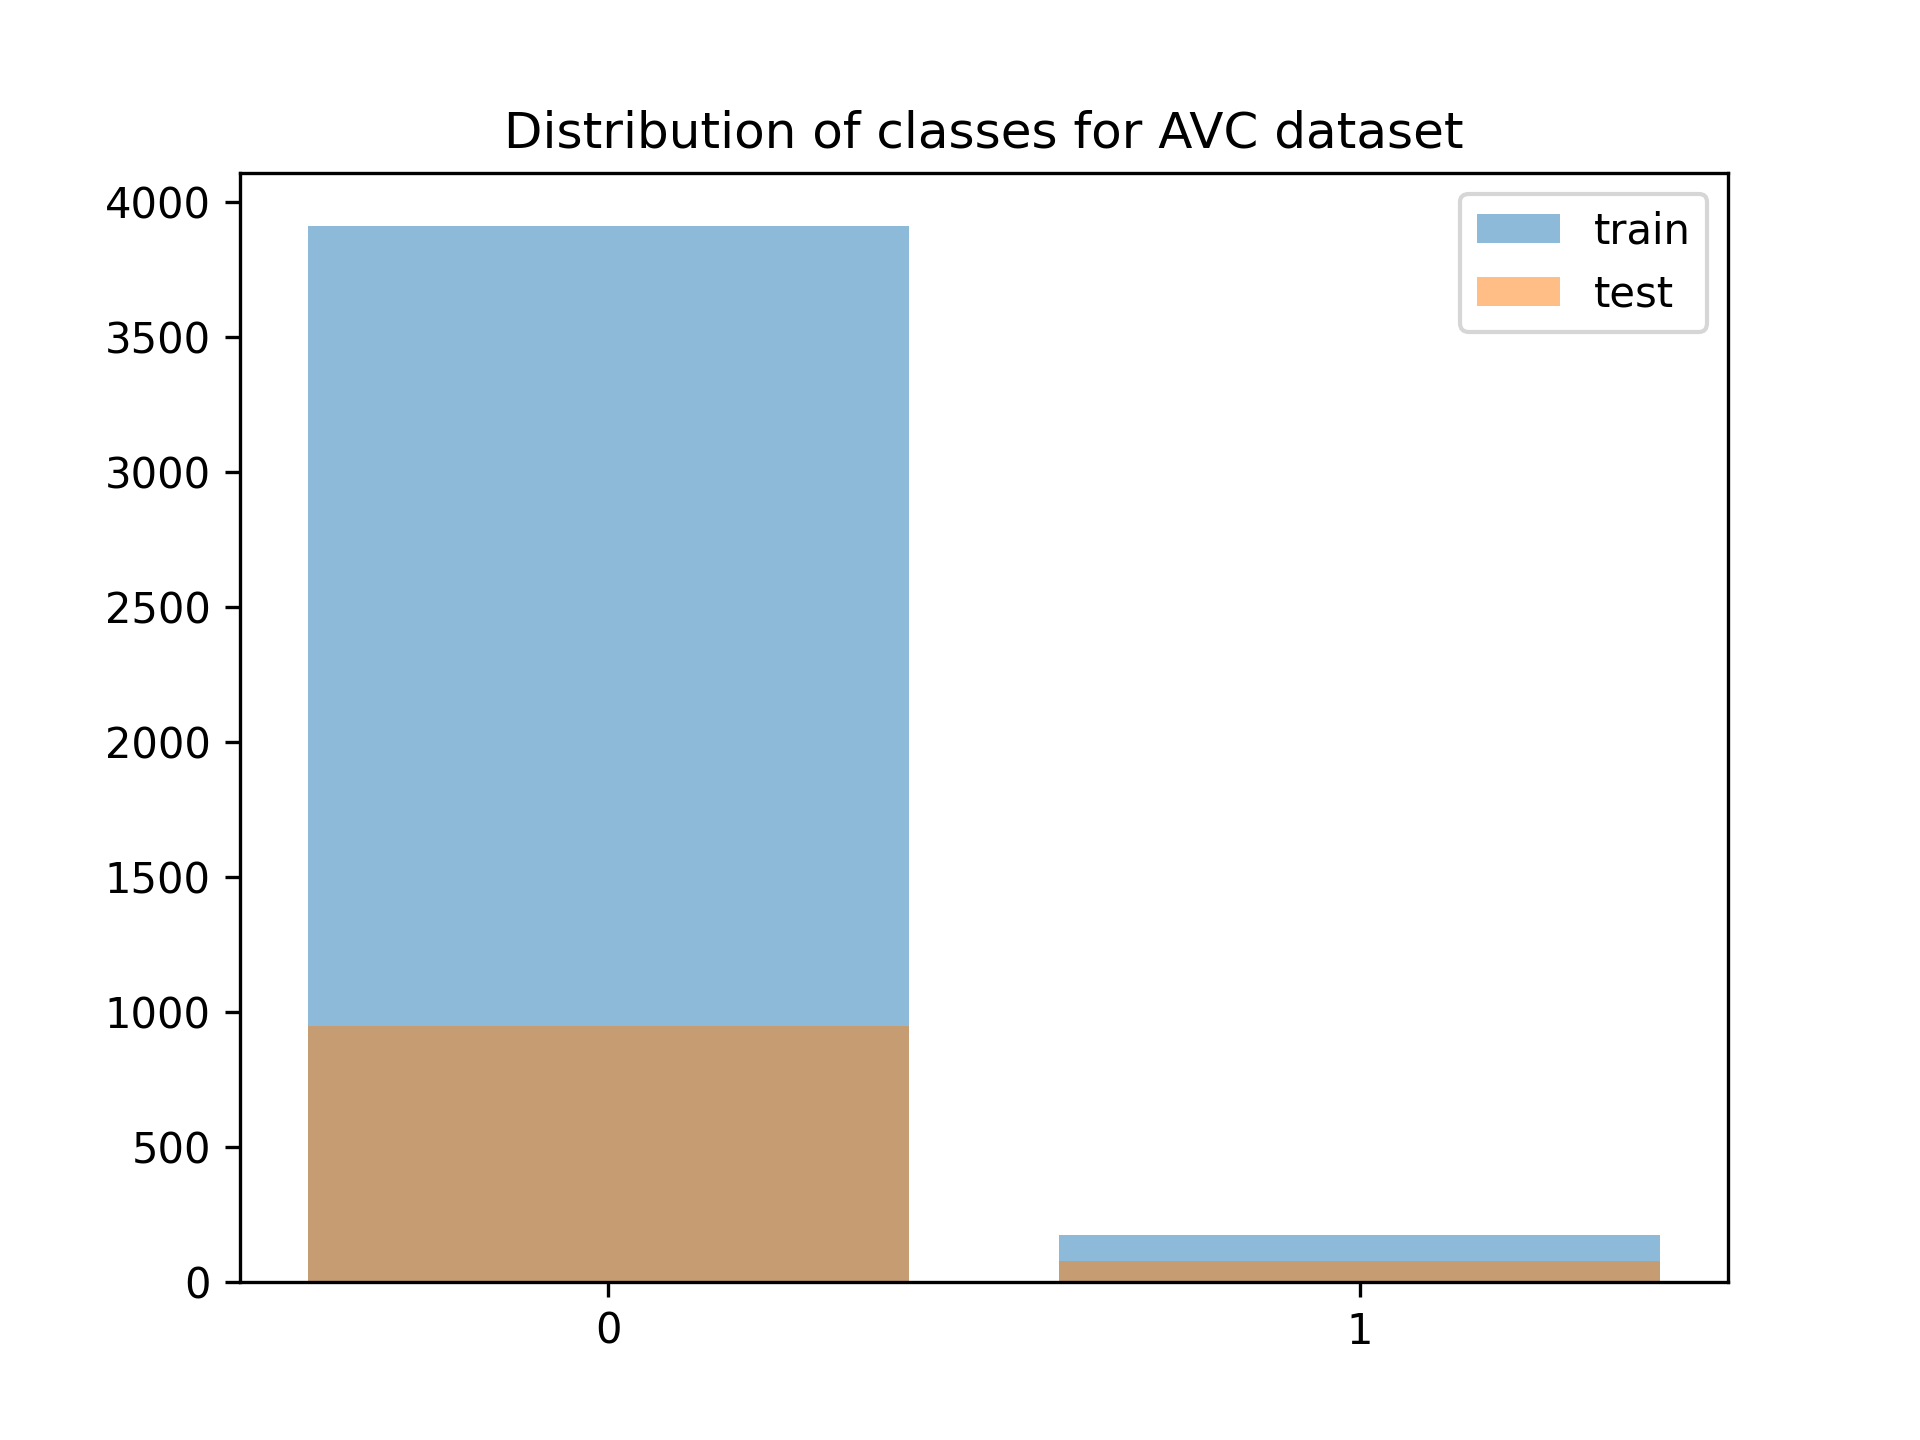
\includegraphics[width=0.8\textwidth]{../plots/distribution_AVC.png}
    \caption{Distribution of the \textit{cerebrovascular\_accident} class in the Stroke Prediction dataset}
    \label{fig:distribution_stroke}
\end{figure}

\subsection{Analysis of Feature Correlations}
Feature correlation analysis is a critical step in understanding the relationships
between different attributes in a dataset. By examining how attributes are related
to each other, we can identify patterns, dependencies, and redundancies that can
inform feature selection, model building, and interpretation.

Correlation analysis typically involves calculating correlation coefficients
between pairs of attributes. The correlation coefficient quantifies the strength
and direction of the linear relationship between two variables. A correlation
coefficient close to 1 indicates a strong positive relationship, while a value
close to -1 indicates a strong negative relationship. A correlation coefficient
near 0 suggests no linear relationship between the variables.

In the \textit{'correlation\_analysis.py'} script, we calculate the correlation
coefficients between all pairs of continuous numeric attributes in the datasets,
generating a correlation matrix for each dataset. Moreover, we calculate the 
Cramér's V coefficient for all pairs of discrete nominal attributes in the datasets,
generating a Cramér's V matrix for each dataset to measure the association between
categorical variables. In Figures \ref{fig:correlation_matrix_example_salary} and
\ref{fig:correlation_matrix_example_stroke} we can see the correlation matrix for
the Salary Prediction and Stroke Prediction datasets, respectively, for the continuous
numeric attributes. In Figures \ref{fig:cramer_v_matrix_example_salary} and
\ref{fig:cramer_v_matrix_example_stroke} we can see the Cramér's V matrix for
the discrete nominal attributes.

\begin{figure}[H]
    \centering
    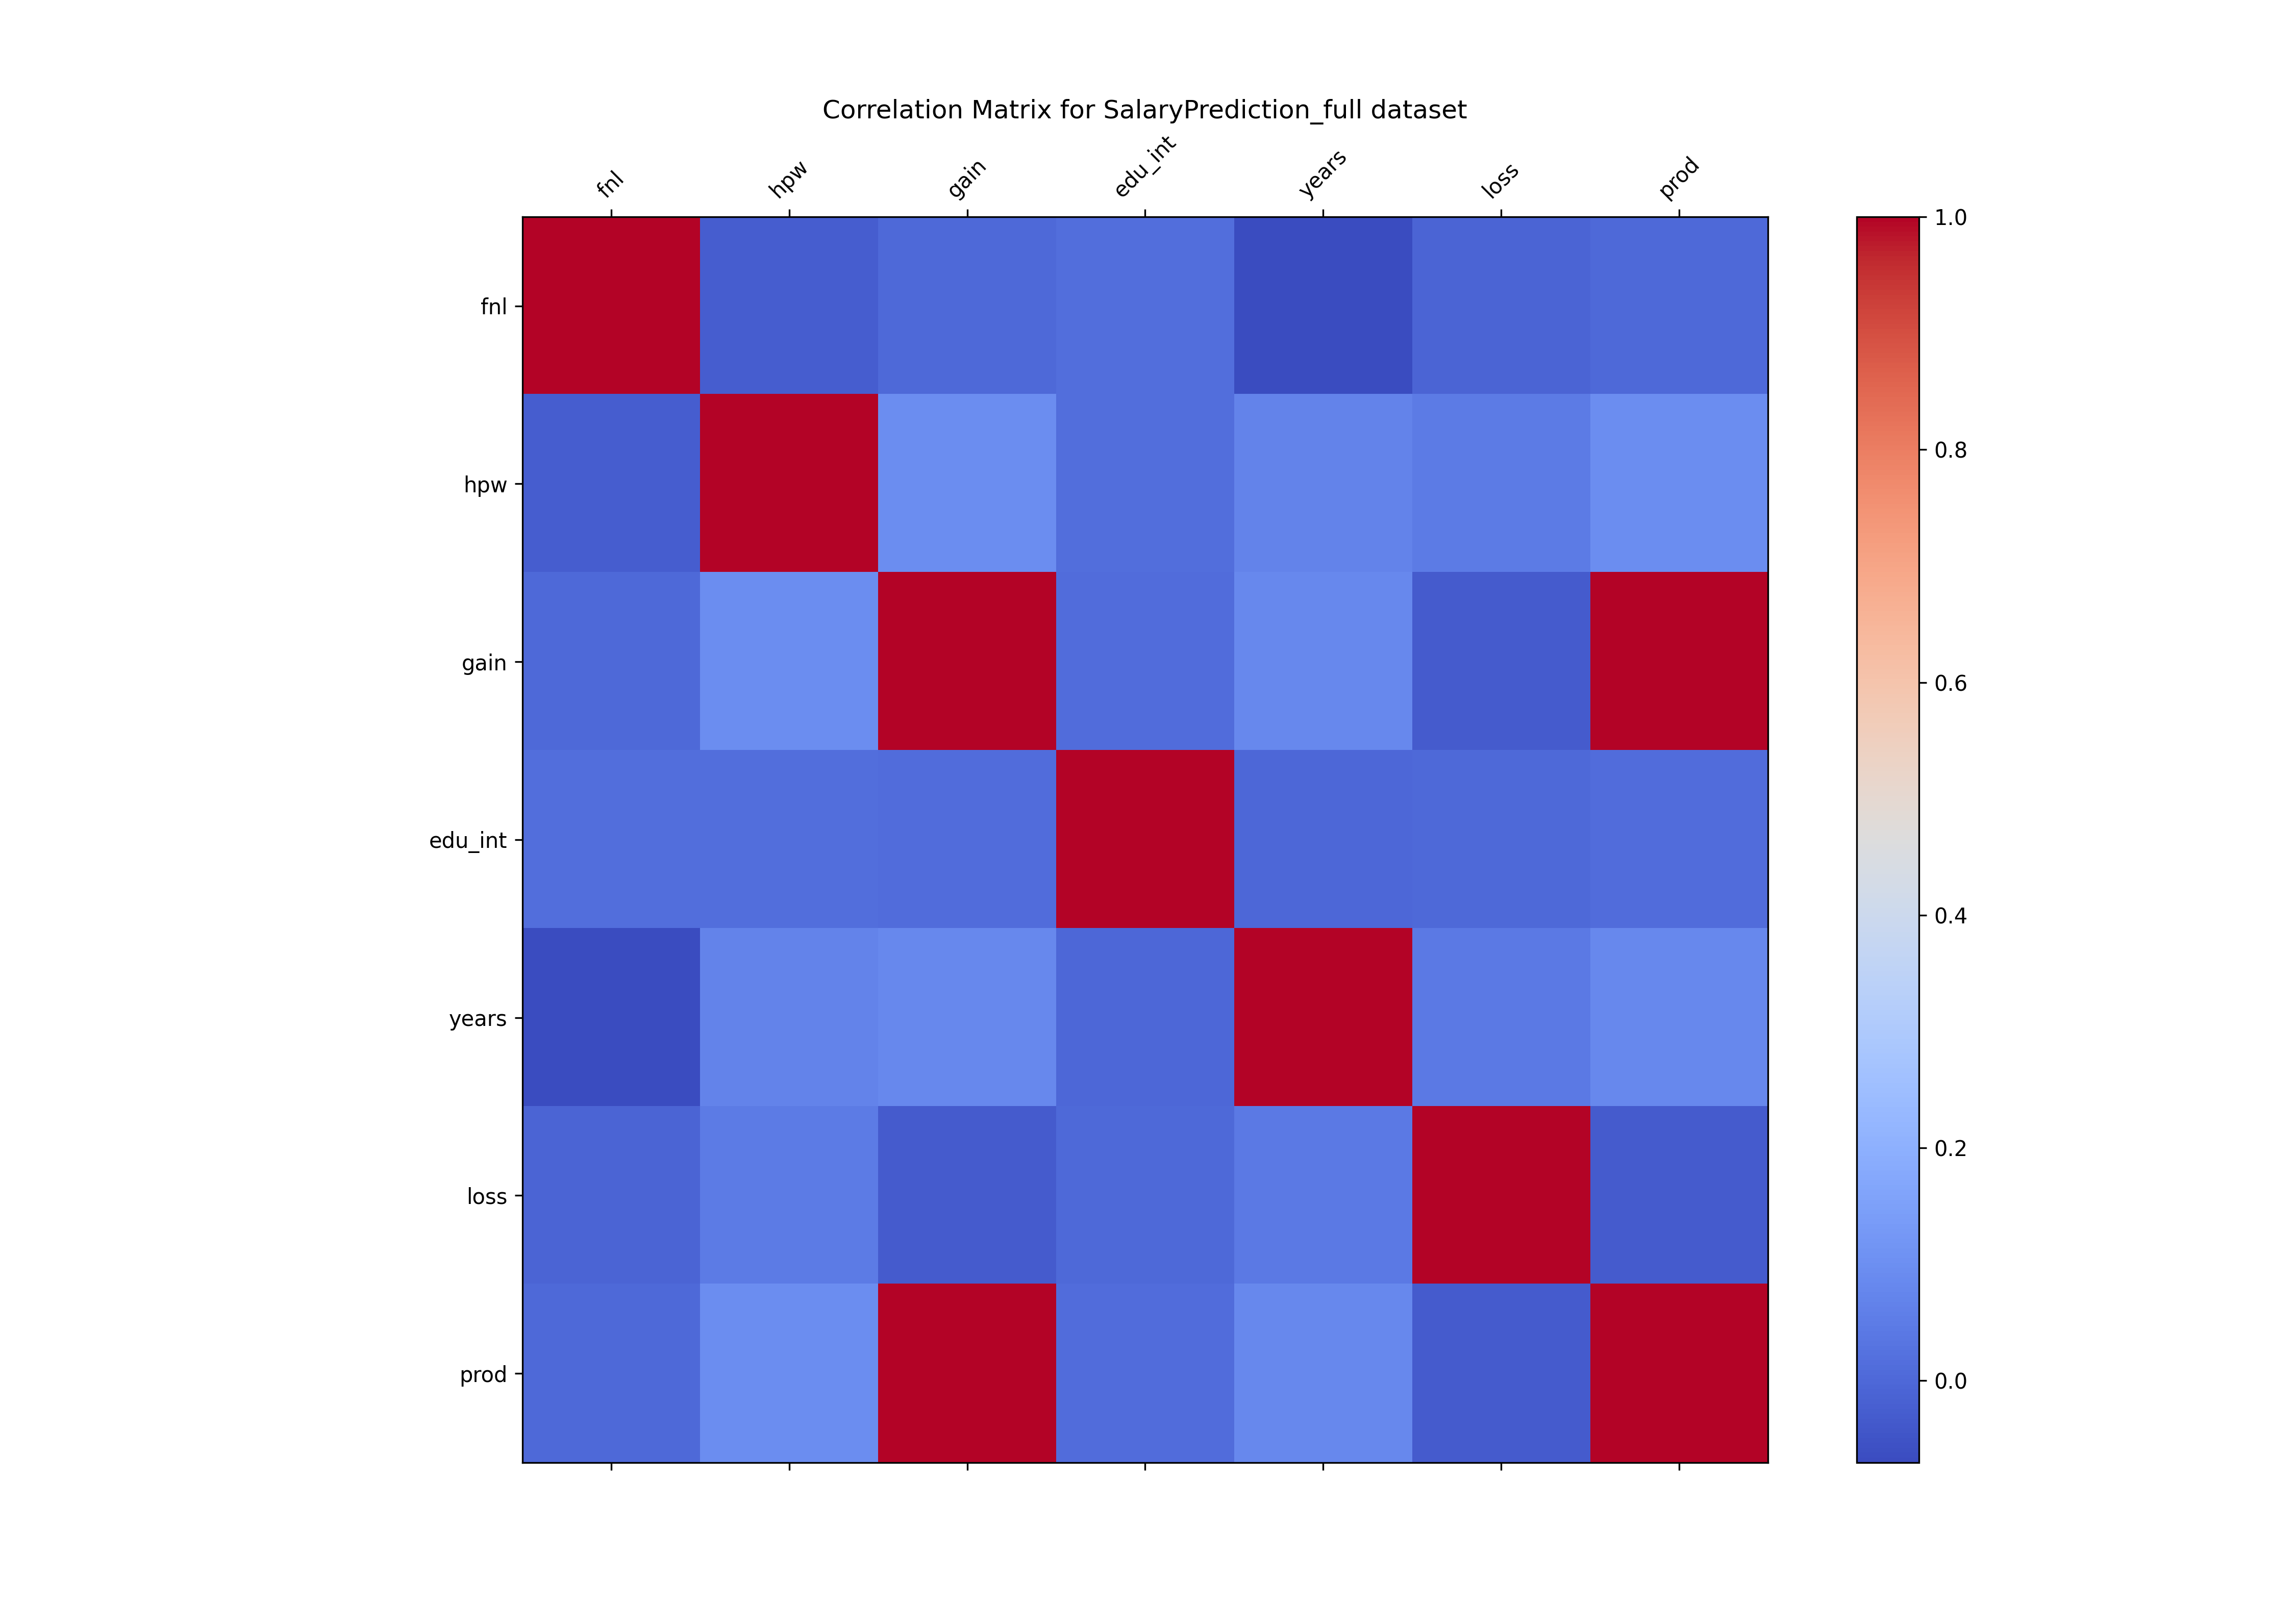
\includegraphics[width=0.8\textwidth]{../plots/correlation_matrix_SalaryPrediction_full.png}
    \caption{Correlation matrix for the Salary Prediction dataset}
    \label{fig:correlation_matrix_example_salary}
\end{figure}
\pagebreak
The correlation matrix and Cramér's V matrix provide valuable insights into the
relationships between attributes in the datasets. By examining these matrices, we
can see that Figure \ref{fig:correlation_matrix_example_salary} the \textit{prod}
attribute is highly correlated with the \textit{gain} attribute, while the
\textit{years} attribute is negatively correlated with the \textit{fnl} attribute.

In Figure \ref{fig:correlation_matrix_example_stroke} we can see that the
\textit{mean\_blood\_sugar\_level} attribute is highly correlated with the
\textit{analysis\_results} attribute, while the \textit{body\_mass\_indicator} 
attribute is negatively correlated with the \textit{analysis\_results} attribute.

\begin{figure}[H]
    \centering
    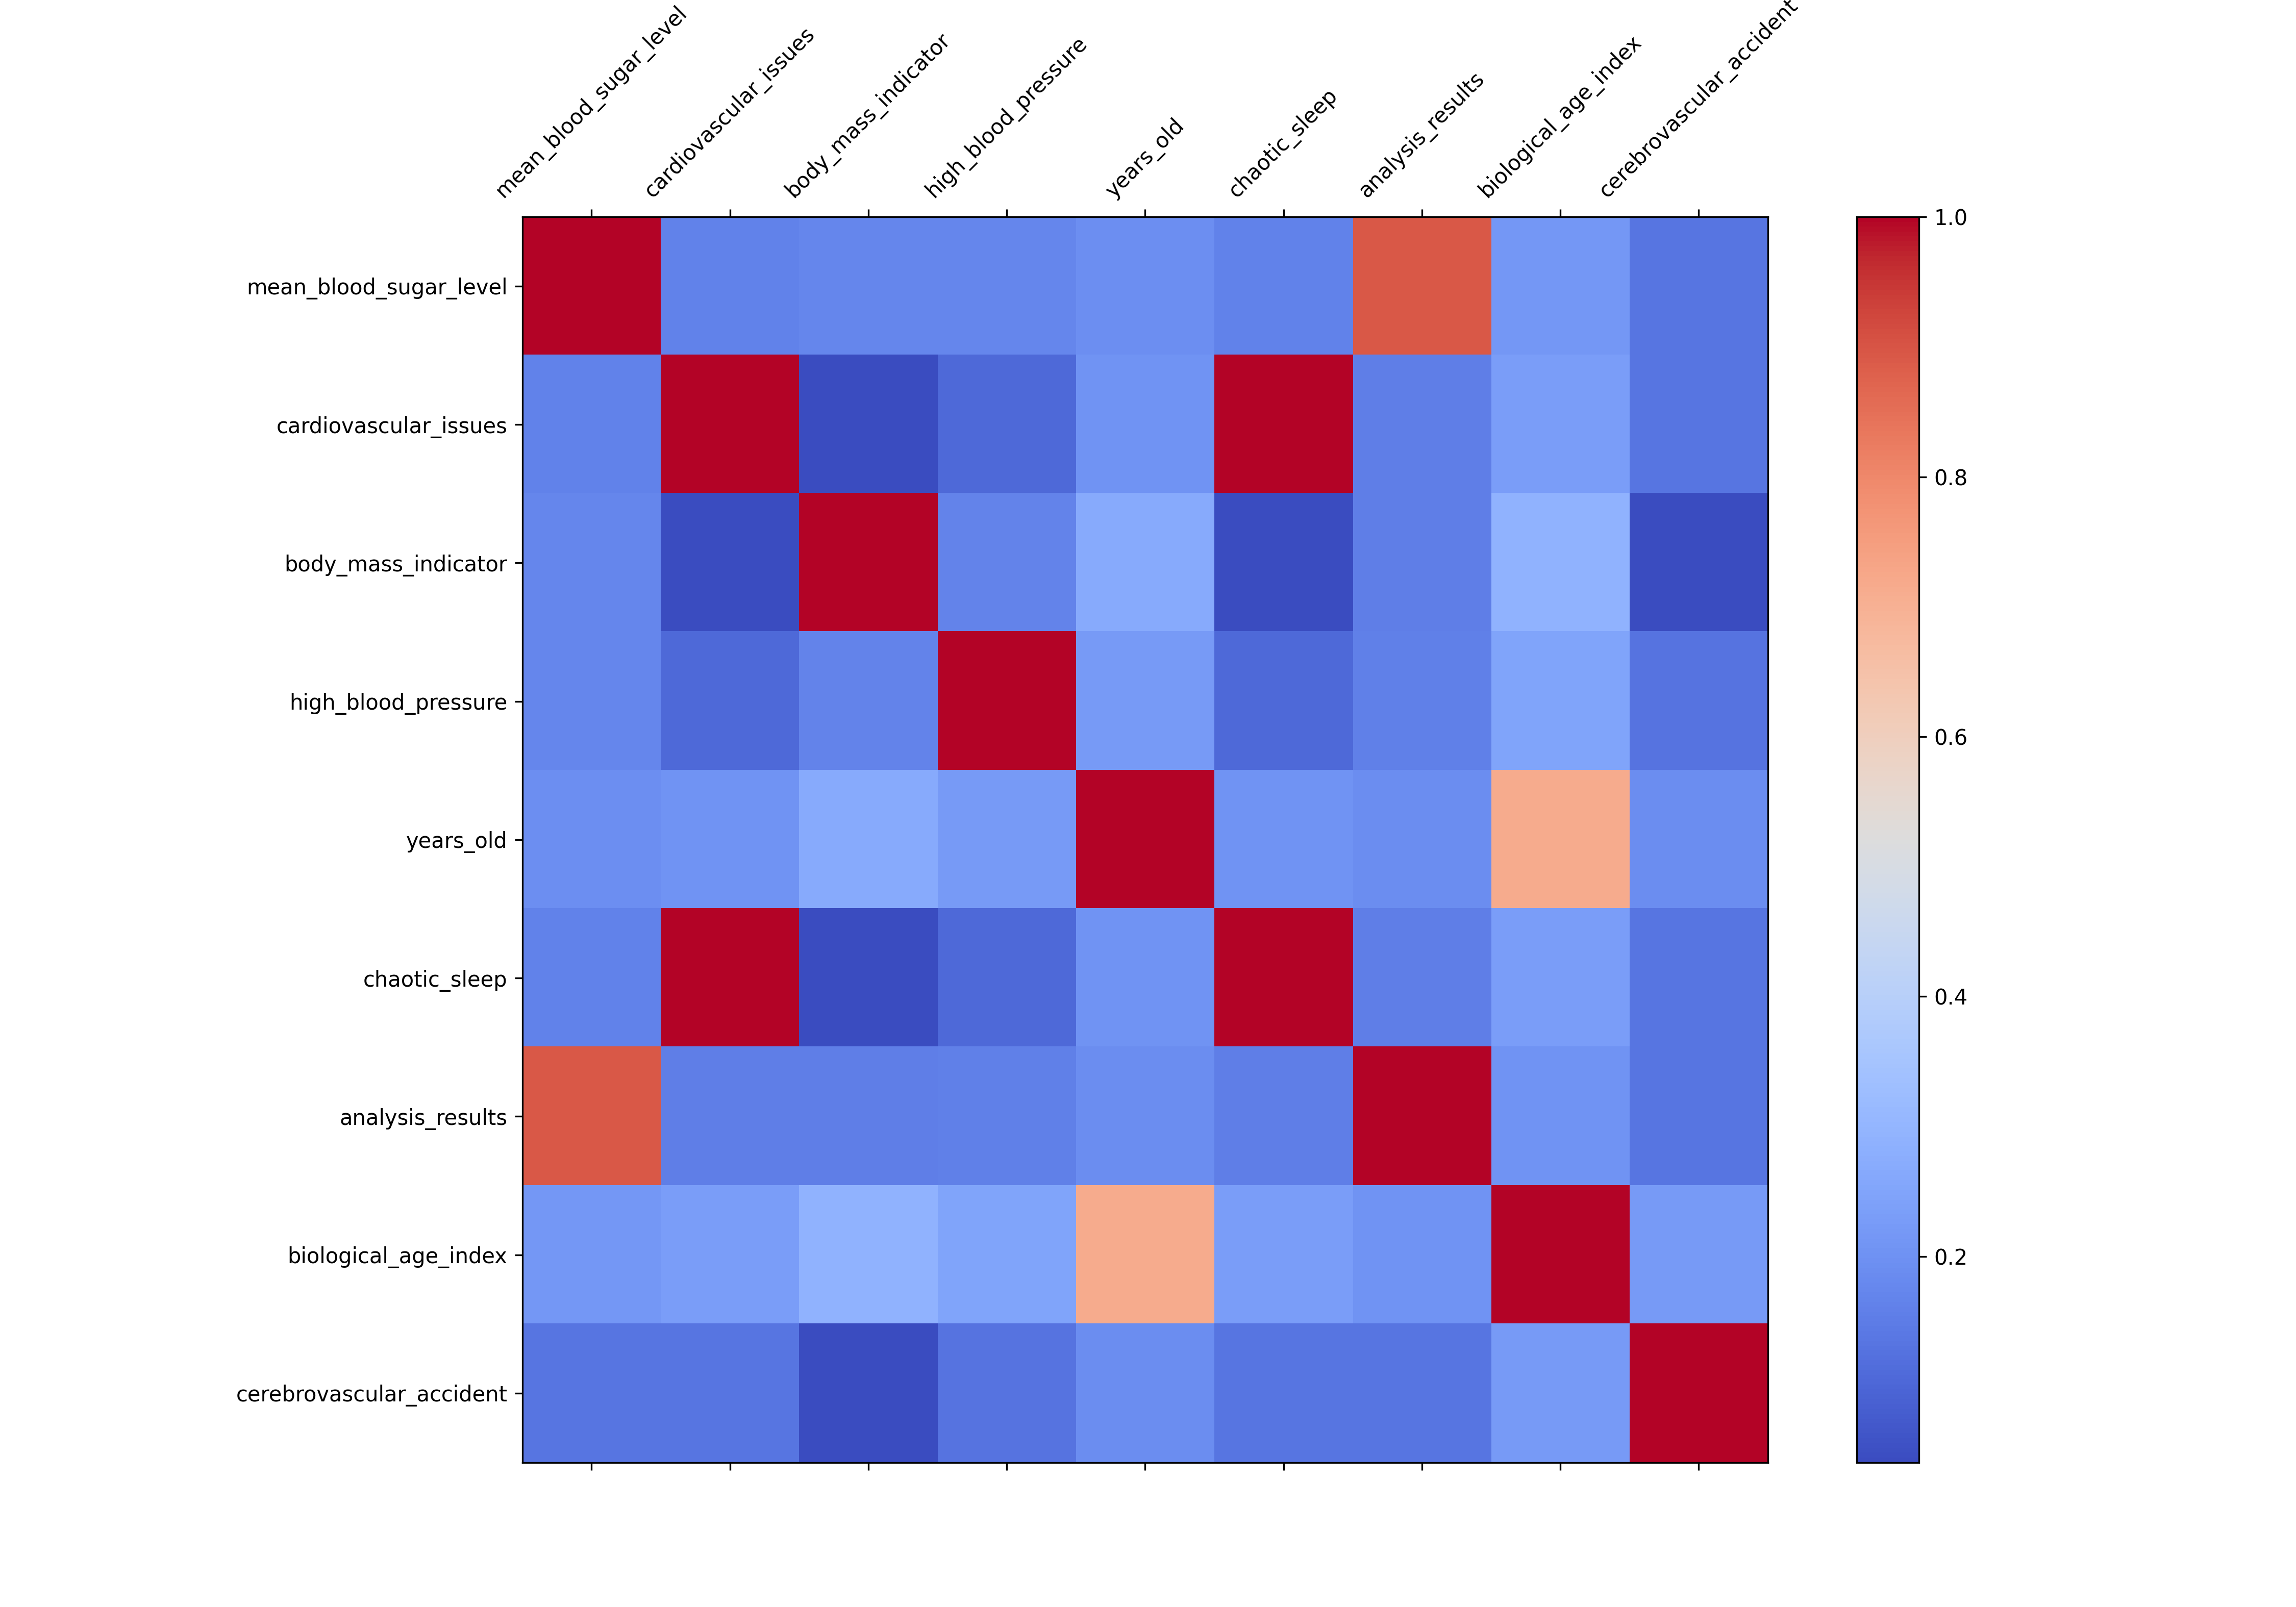
\includegraphics[width=0.8\textwidth]{../plots/correlation_matrix_AVC_full.png}
    \caption{Correlation matrix for the Stroke Prediction dataset}
    \label{fig:correlation_matrix_example_stroke}
\end{figure}

The Cramér's V matrix in Figures \ref{fig:cramer_v_matrix_example_salary} and
\ref{fig:cramer_v_matrix_example_stroke} provides insights into the association
between discrete nominal attributes. For example, in the Salary Prediction dataset,
the \textit{gtype} attribute is strongly associated with the \textit{gender} attribute,
while in the Stroke Prediction dataset, the \textit{cardiovascular\_issues} attribute is strongly
associated with the \textit{chaotic\_sleep} attribute.

\begin{figure}[H]
    \centering
    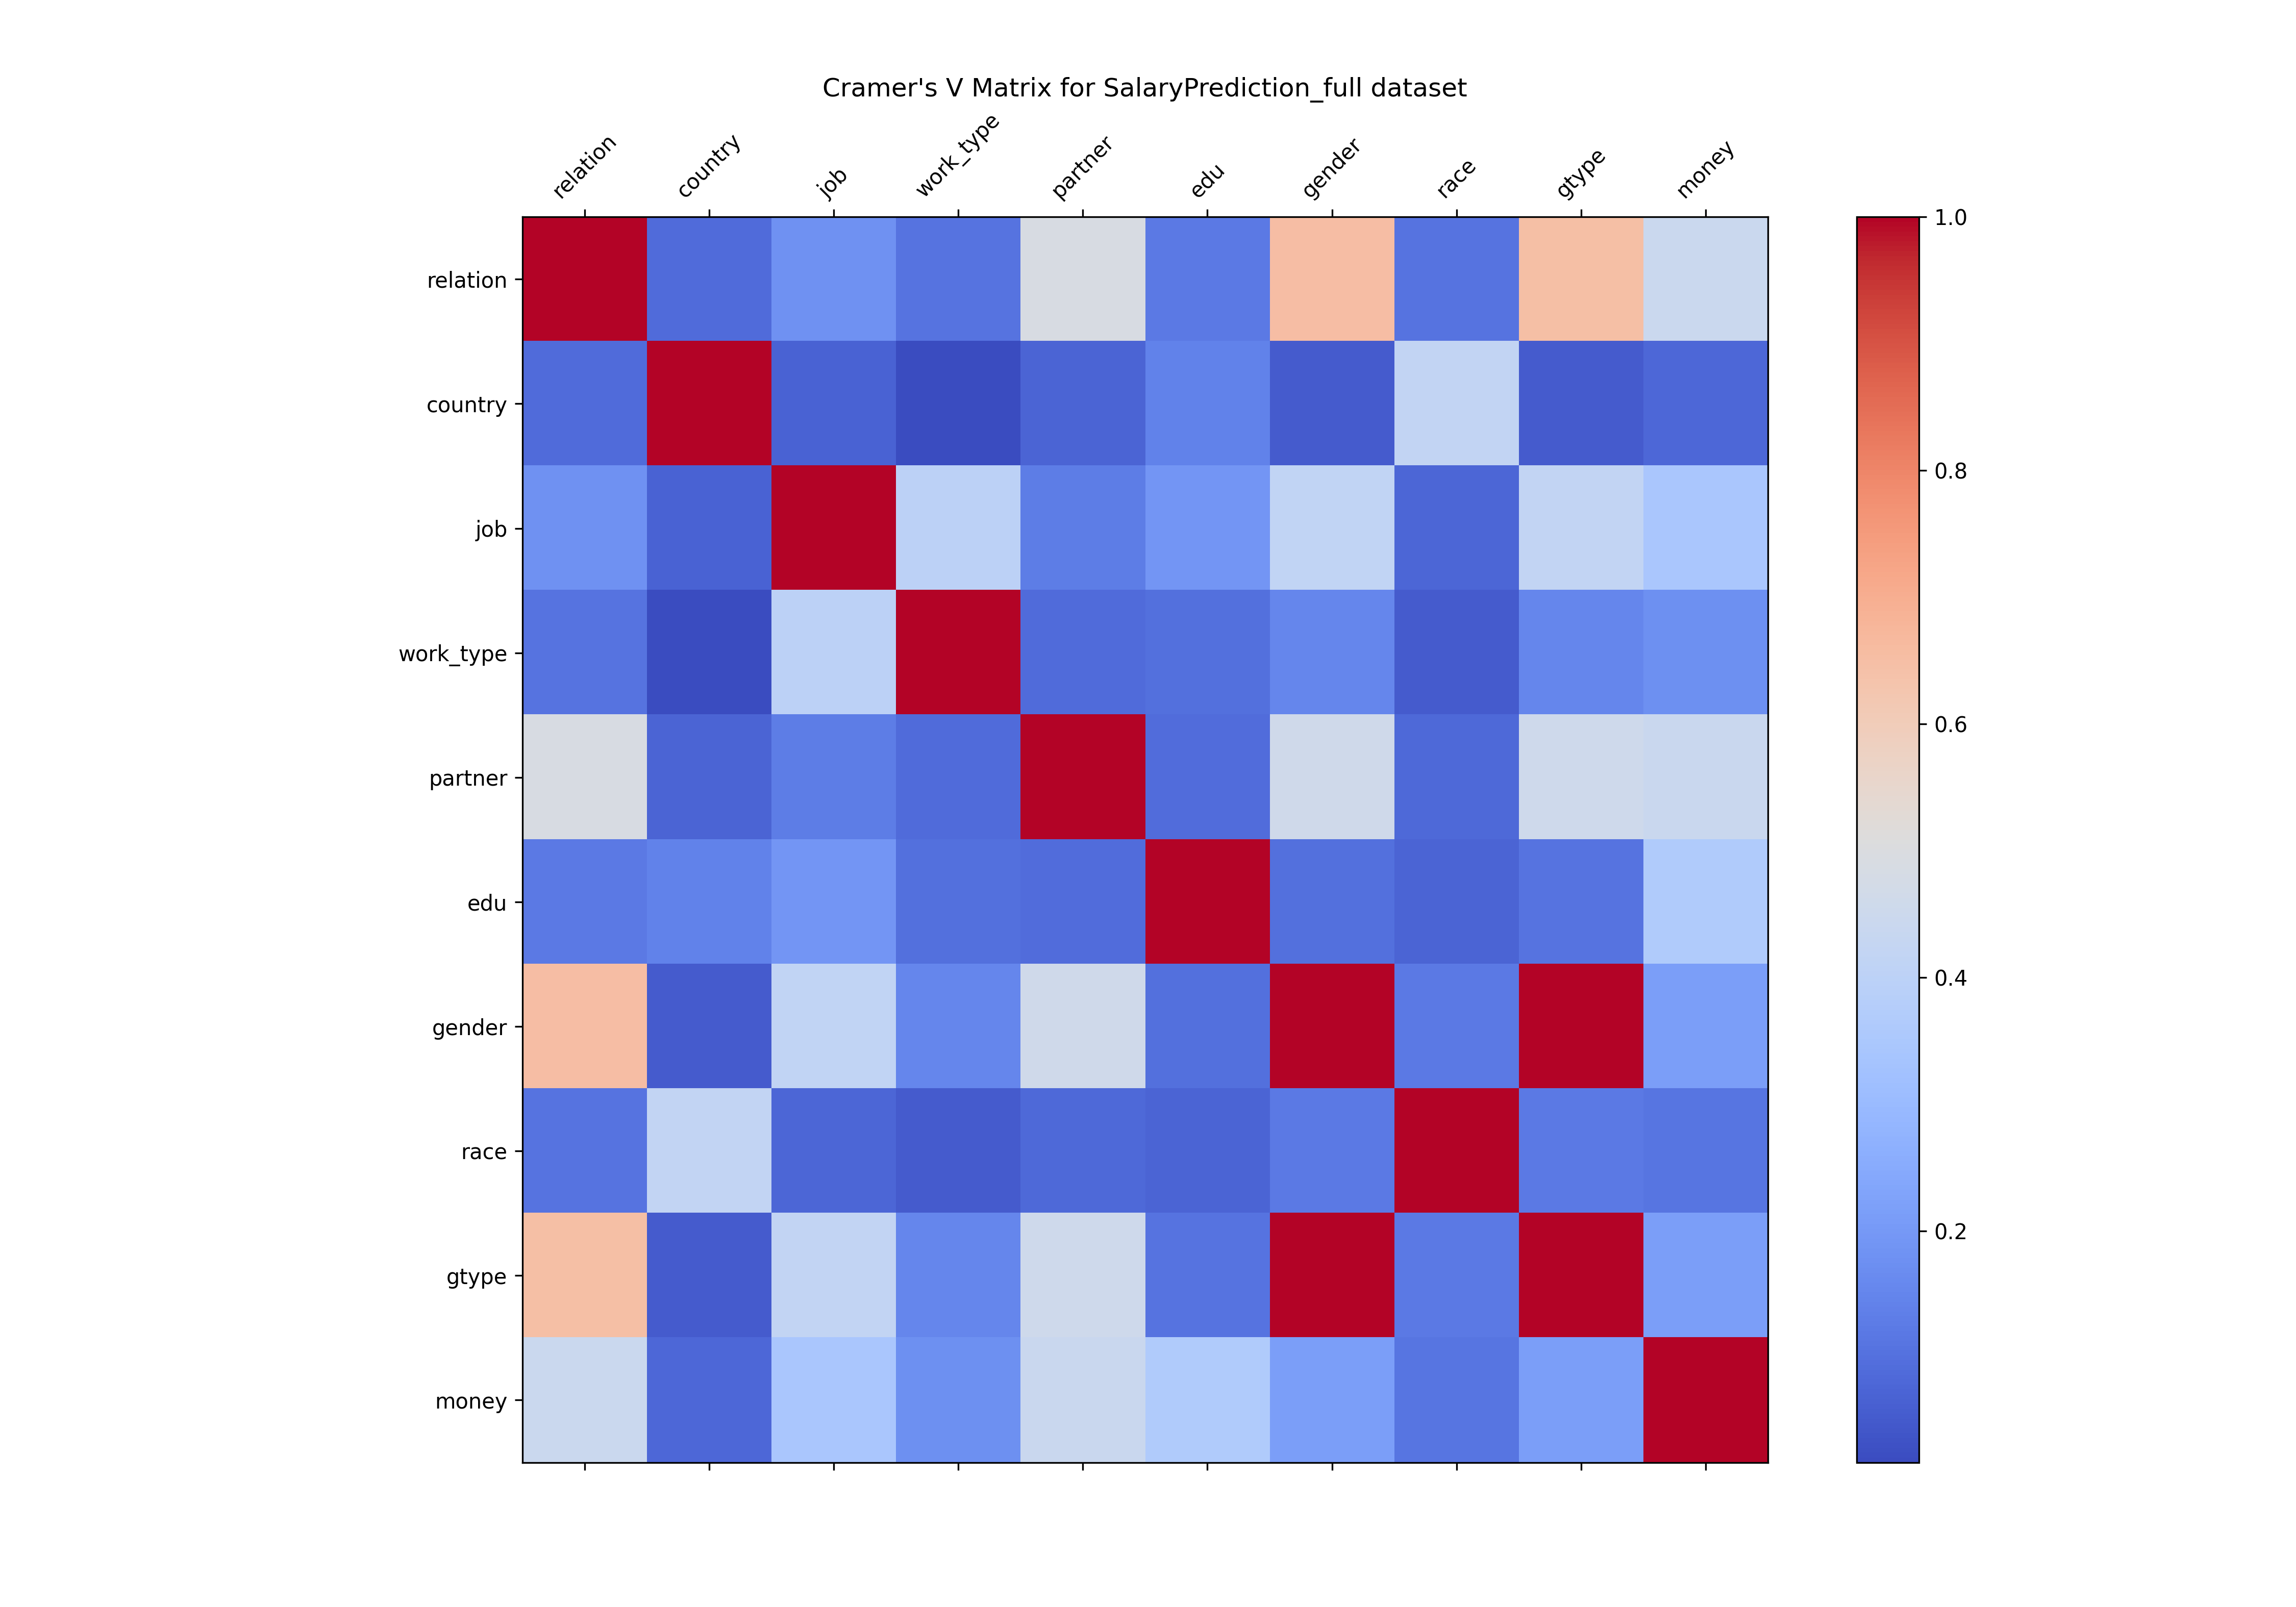
\includegraphics[width=0.8\textwidth]{../plots/cramer_v_matrix_SalaryPrediction_full.png}
    \caption{Cramér's V matrix for the Salary Prediction dataset}
    \label{fig:cramer_v_matrix_example_salary}
\end{figure}

\begin{figure}[H]
    \centering
    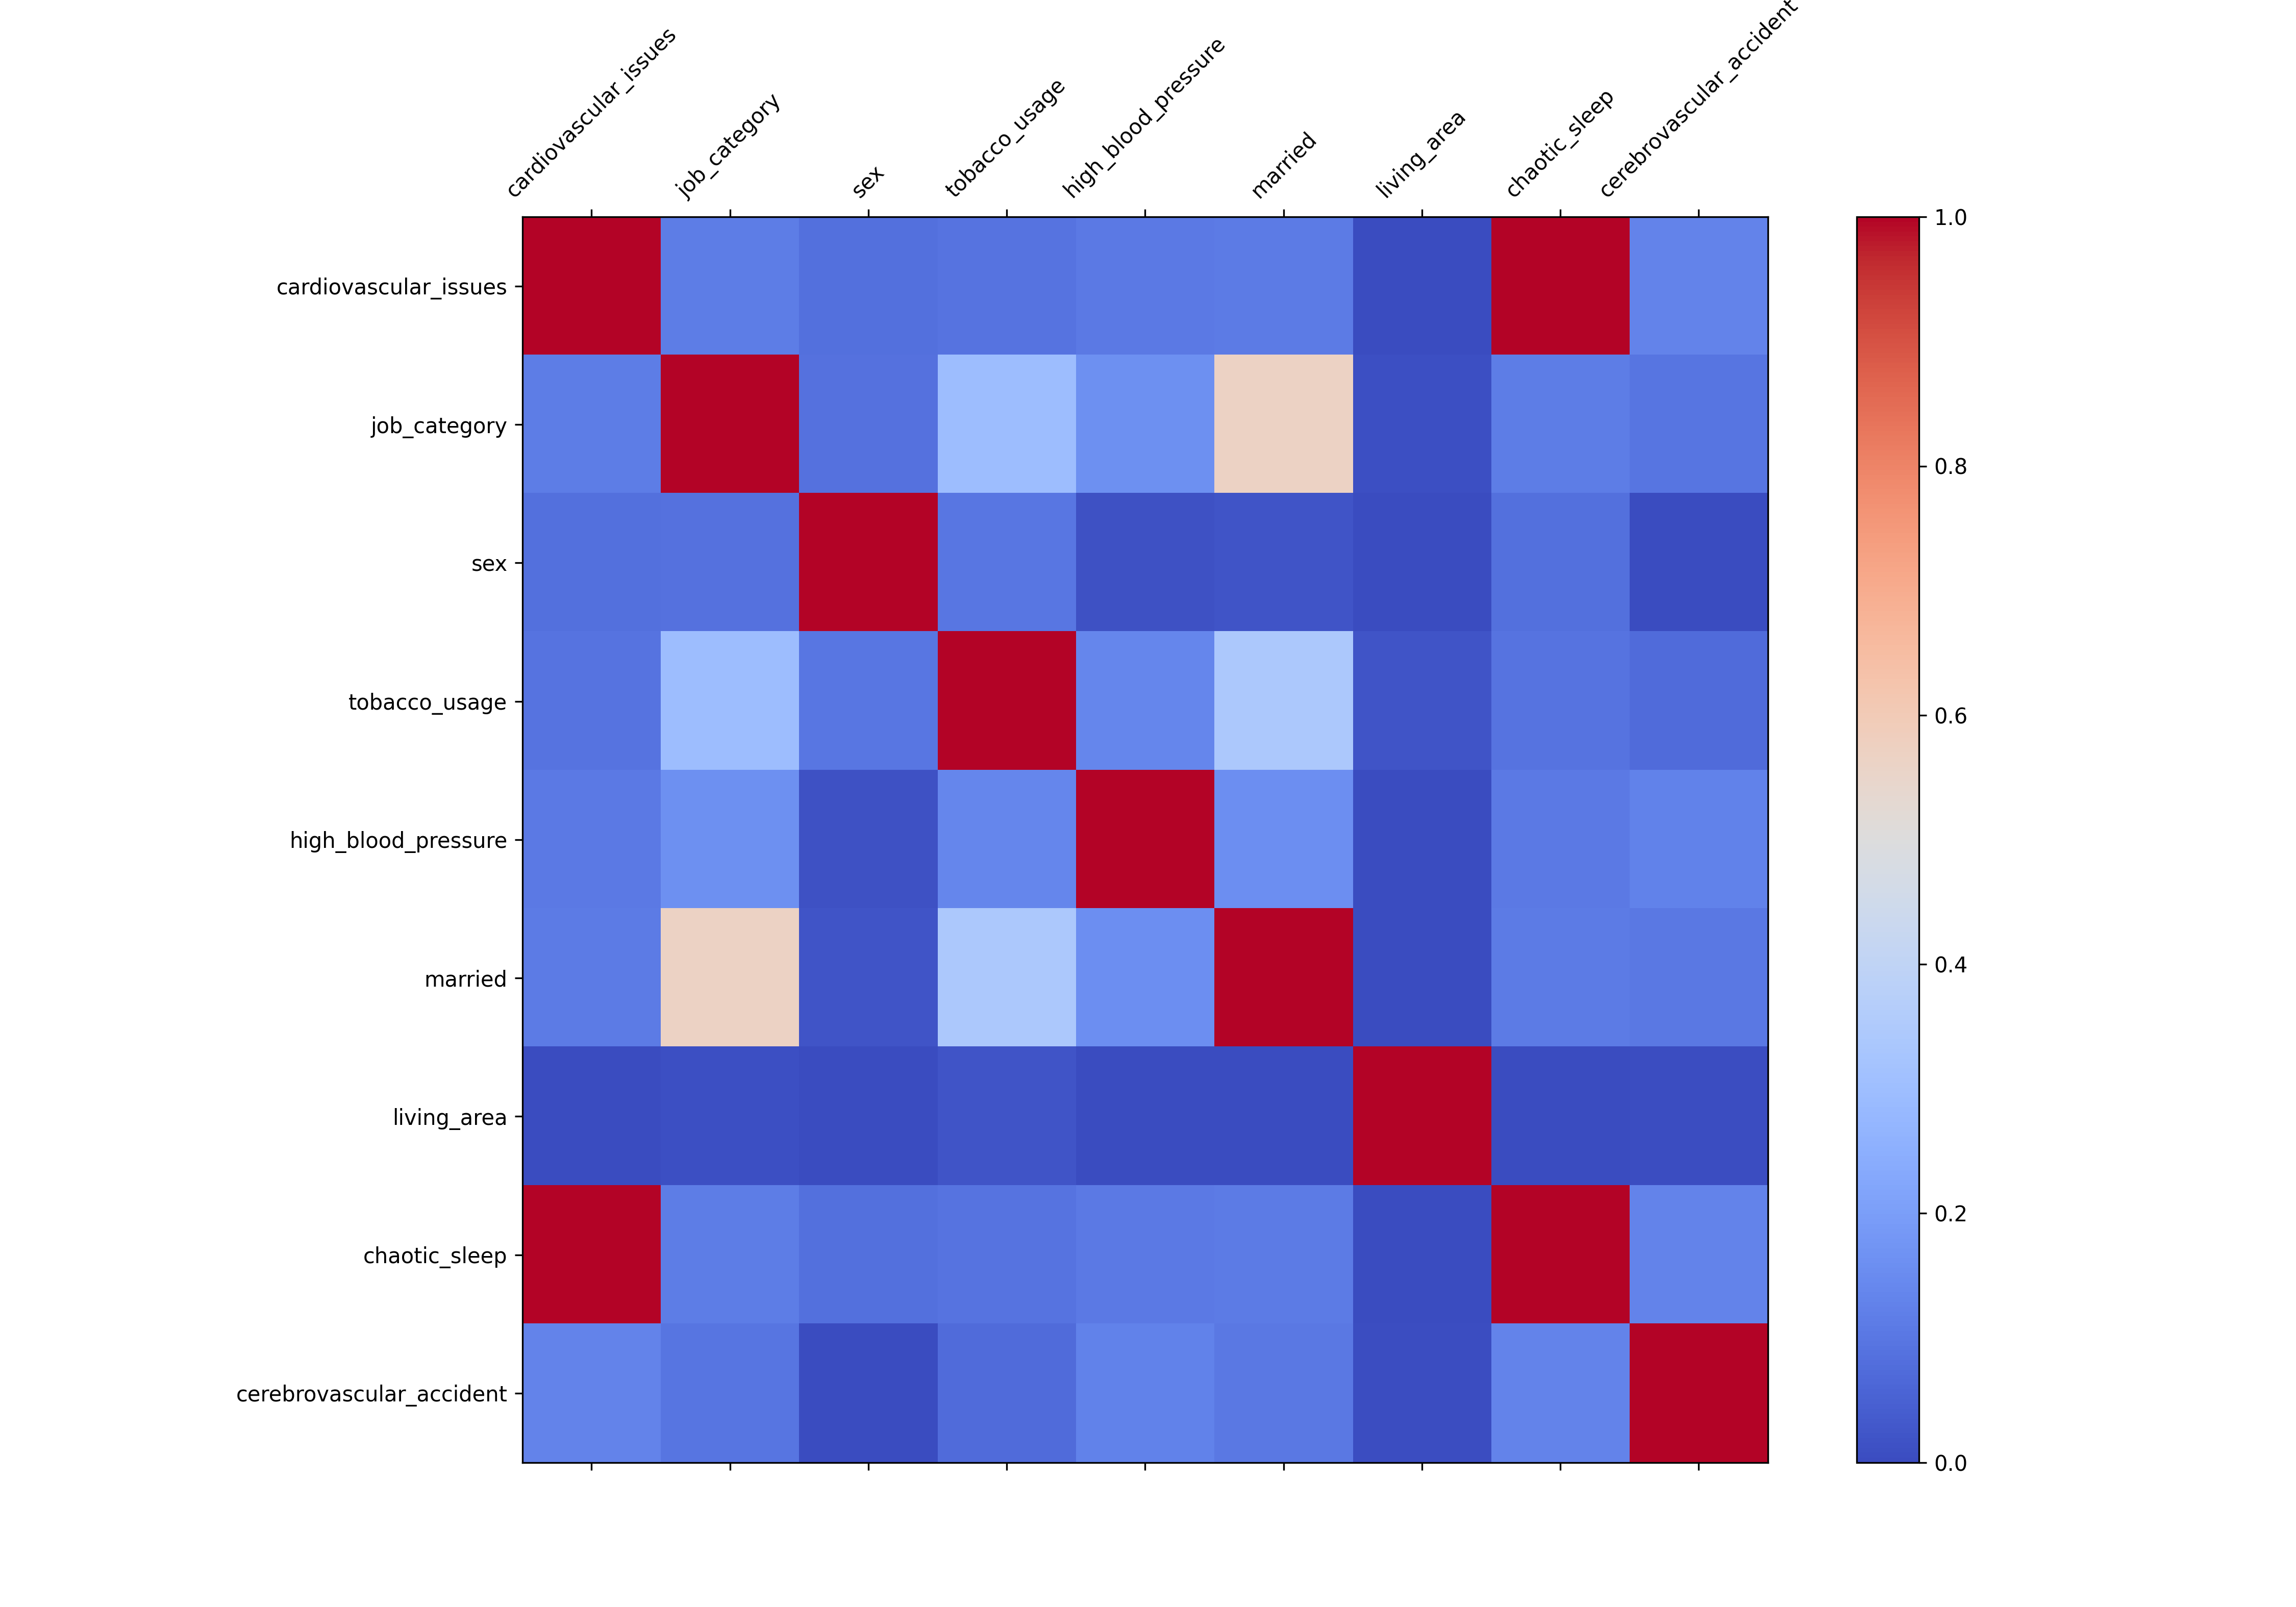
\includegraphics[width=0.8\textwidth]{../plots/cramer_v_matrix_AVC_full.png}
    \caption{Cramér's V matrix for the Stroke Prediction dataset}
    \label{fig:cramer_v_matrix_example_stroke}
\end{figure}

% ------------------------------------------------------------------------------
\section{Data Preprocessing}
As highlighted in the previous section, high-quality data is the cornerstone of 
effective machine learning models. However, real-world datasets often exhibit 
various imperfections that can impede model performance.  Our exploration of the 
datasets revealed the presence of several such issues, including:

\begin{itemize}
    \item Missing values for specific attributes.
    \item Extreme values (outliers) within certain attributes.
    \item Redundant attributes with high correlation.
    \item Inconsistent value ranges for numeric attributes.
\end{itemize}

These imperfections necessitate data preprocessing, a crucial step aimed at 
transforming the raw data into a clean and consistent format. This section 
delves into the specific data preprocessing techniques employed in this study. 
By addressing these issues, we aim to optimize the data for subsequent machine 
learning algorithms, ultimately enhancing their effectiveness in extracting 
valuable insights. 

As a note, all the scripts for data preprocessing are located in the \textit{'preprocessing'}
folder at the root of the project directory.

\subsection{Handling Missing Values}
Missing data, a common issue in real-world datasets, necessitates the application
of imputation procedures to address these missing values.  Imputation techniques 
can be categorized as either univariate or multivariate:

\begin{itemize}
    \item \textit{Univariate Imputation:} This approach focuses solely on the attribute with missing 
    values. Common univariate techniques include replacing missing values with the 
    mean, median, or most frequent value within the attribute. These methods are 
    simple to implement but may not effectively capture the underlying relationships 
    between attributes.
    \item \textit{Multivariate Imputation:} This more sophisticated approach leverages the values 
    of other attributes within a sample to estimate the missing value. Techniques 
    like regression analysis are often employed to establish relationships between 
    the missing attribute and the remaining attributes. Based on these relationships, 
    a predicted value can be imputed for the missing data point.  Multivariate 
    imputation offers a more nuanced approach but requires careful consideration 
    of the relationships between attributes and potential biases in the imputation 
    process.
\end{itemize}

In the \textit{'impute\_values.py'} script, in the \textit{'missing\_values'} function,
we used the \textit{IterativeImputer}
class from the \textit{sklearn.impute} module to apply multivariate imputation to
address missing values in the datasets for continuous numeric attributes. The script
uses the most frequent value strategy for categorical attributes. The imputed datasets
are saved in the same folder as the original datasets, with the prefix
\textit{'preprocessed\_missing\_'}.

\subsection{Outlier Detection and Treatment}
Outliers, data points that deviate significantly from the rest of the dataset,
can adversely affect the performance of machine learning models. Outliers can
skew statistical measures, distort relationships between attributes, and lead to
poor generalization of the model. Detecting and treating outliers is essential
for ensuring the robustness and reliability of the model.

We purpose to impute the outliers using the \textit{IsolationForest} algorithm
from the \textit{sklearn.ensemble} module. The script \textit{'outlier\_detection.py'}
detects outliers in the continuous numeric attributes of the datasets and replaces
them with the imputed values. The preprocessed datasets with imputed outliers are
saved in the same folder as the original datasets, with the prefix
\textit{'preprocessed\_outliers\_'}.

\subsection{Analysis of Attribute Correlations}
As previously discussed, attribute correlations can provide valuable insights
into the relationships between different attributes in the dataset. By identifying
highly correlated attributes, we can eliminate redundant information and reduce
the dimensionality of the data, leading to more efficient model training and
improved interpretability.

We choose to remove highly correlated attributes found in the section of
Exploratory Data Analysis. These attributes are:

\begin{itemize}
    \item \textit{prod}: it is correlated with \textit{gain} in the Salary Prediction dataset.
    \item \textit{analysis\_results}: it is correlated with \textit{body\_mass\_indicator} in the Stroke Prediction dataset.
    \item \textit{gtype}: it is correlated with \textit{gender} in the Salary Prediction dataset.
    \item 
\end{itemize}

The script \textit{'remove\_correlated\_attributes.py'}
removes those attributes from the train dataset and saves the preprocessed dataset
in the same folder as the original datasets, with the prefix \textit{'preprocessed\_correlated\_'}.

\subsection{Normalization and Standardization}
The numerical attributes in the dataset can vary significantly in their value scales. For example, 
some attributes may have values in the thousands, while others have values in the single digits. 
This disparity in scales can significantly affect algorithms like Logistic Regression.

In algorithms like Logistic Regression, which rely on a linear combination of attribute values,
attributes with larger numerical values can disproportionately influence the model. This dominance 
can lead to biased results and reduce the model's effectiveness.

To mitigate this issue, it is essential to standardize the values of the numeric attributes. 
Standardization adjusts the scales of the attributes, ensuring that each one contributes equally 
to the model's predictions. This process improves the performance and accuracy of the model by 
creating a more balanced and fair representation of the data.

% ------------------------------------------------------------------------------
\section{Algorithms Designs}
Algorithm design is a critical aspect of computer science and machine learning, 
focusing on creating efficient and effective methods to solve complex problems. 
The process involves the careful selection of algorithms based on the specific 
characteristics of the data and the desired outcomes. This document explores the 
application of two prominent machine learning algorithms, Linear Regression and 
Multi-Layered Perceptron (MLP), on diverse datasets. The goal is to compare their 
performance and suitability for different types of prediction tasks, particularly 
in the contexts of stroke prediction and salary prediction.

\subsection{Linear Regression}
Linear Regression is one of the most fundamental and widely used algorithms in 
machine learning. It is known for its simplicity, interpretability, and 
efficiency in identifying linear relationships between variables. The primary 
purpose of Linear Regression is to model the relationship between a dependent 
variable and one or more independent variables by fitting a linear equation to 
observed data.

In the context of stroke prediction, Linear Regression can be used to analyze 
how various factors such as age, blood pressure, cholesterol levels, and smoking 
history influence the likelihood of experiencing a stroke. Its straightforward 
approach allows for clear insights into the significance and impact of each 
factor on stroke risk.

In the \textit{linear\_regression} folder at the root of the project directory,
we implemented the Linear Regression algorithm in two different ways:

\begin{itemize}
    \item \textit{Linear Regression with Scikit-Learn:} We used the Scikit-Learn
    library to implement Linear Regression on the preprocessed datasets.
    \item \textit{Linear Regression from Scratch:} We implemented Linear Regression
    as in the 8th laboratory from the Artificial Intelligence course.
\end{itemize}

I choose to implement the RidgeRegression algorithm. Because of the large number of
features in the dataset, the RidgeRegression algorithm is more suitable than the
LinearRegression algorithm. The RidgeRegression algorithm is a regularized version
of Linear Regression that adds a penalty term to the loss function to prevent overfitting.
This penalty term helps to reduce the model's complexity and improve its generalization
performance. The alpha parameter controls the strength of the regularization, with
higher values of alpha leading to stronger regularization. I used the value of alpha
1.75 because it provided the best results in the experiments.

For enconding the categorical attributes except the target attribute, I used the
\textit{OneHotEncoder} class from the \textit{sklearn.preprocessing} module. This
class encodes categorical attributes as one-hot vectors, creating a binary representation
of each category. This encoding is essential for feeding categorical attributes into
machine learning models, as most algorithms require numerical input data. For the
target attribute, I used the \textit{LabelEncoder} class from the \textit{sklearn.preprocessing}
module to encode the target attribute as integer values.

The results of both implementations for each dataset are saved in the \textit{LinearRegression}
folder at the specific dataset's root.

\subsection{Multi-Layered Perceptron (MLP)}
Multi-Layer Perceptron (MLP) is a type of artificial neural network designed to 
capture complex, non-linear patterns in data. Unlike Linear Regression, which is
limited to linear relationships, MLPs consist of multiple layers of interconnected 
nodes, or neurons, that can model intricate interactions between variables.

MLPs are particularly suitable for tasks involving complex datasets with 
non-linear relationships, such as salary prediction. In salary prediction, 
factors like education, work experience, industry sector, and other 
socio-economic variables interact in complex ways that Linear Regression might 
not fully capture. MLPs can learn these non-linear patterns, providing a more 
accurate and nuanced understanding of the factors influencing salary levels.

% ------------------------------------------------------------------------------

\section{Evaluation}

% ------------------------------------------------------------------------------
\section{Conclusions}


\pagebreak
% ------------------------------------------------------------------------------

% ---- Bibliography ----
\begin{thebibliography}{8}
    \bibitem{}
    \href{https://curs.upb.ro/2023/course/view.php?id=13749}{Moodle - Artifical Intelligence Course}
    \bibitem{}
    \href{https://en.wikipedia.org/wiki/Linear_regression}{Wikipedia - Linear Regression}
    \bibitem{}
    \href{https://en.wikipedia.org/wiki/Linear_classifier}{Wikipedia - Linear Classifier}
    \bibitem{}
    \href{https://en.wikipedia.org/wiki/Ridge_regression}{Wikipedia - Ridge Regression}
    \bibitem{}
    \href{https://www.semanticscholar.org/reader/2c9022fe0af15568a885e59d475ec8f95726e51b}{Metrics for Multi-Class Classification: An Overview}
    \bibitem{}
    \href{https://pandas.pydata.org/docs/reference/api/pandas.DataFrame.html}{Pandas - DataFrame}
    \bibitem{}
    \href{https://en.wikipedia.org/wiki/Correlation}{Wikipedia - Correlation}
    \bibitem{}
    \href{https://thinkingneuron.com/how-to-measure-the-correlation-between-two-categorical-variables-in-python/}{Thinking Neuron - How to Measure the Correlation Between Two Categorical Variables in Python}
    \bibitem{}
    \href{https://www.stratascratch.com/blog/chi-square-test-in-python-a-technical-guide/}{StrataScratch - Chi-Square Test in Python: A Technical Guide}
    \bibitem{}
    \href{https://en.wikipedia.org/wiki/Cram\%C3\%A9r\%27s\_V}{Wikipedia - Cramér's V}
    \bibitem{}
    \href{https://saturncloud.io/blog/how-to-detect-and-exclude-outliers-in-a-pandas-dataframe/}{Saturn Cloud - How to Detect and Exclude Outliers in a Pandas DataFrame}
    \bibitem{}
    \href{https://www.kaggle.com/discussions/questions-and-answers/159183}{Kaggle - When to standardize test and train data?}
    \bibitem{}
    \href{https://scikit-learn.org/stable/modules/preprocessing.html#standardization-or-mean-removal-and-variance-scaling}{Scikit-Learn - Standardization or Mean Removal and Variance Scaling}
    \bibitem{}
    \href{https://scikit-learn.org/stable/modules/generated/sklearn.preprocessing.OneHotEncoder.html}{Scikit-Learn - OneHotEncoder}
    \bibitem{}
    \href{https://scikit-learn.org/stable/modules/generated/sklearn.preprocessing.LabelEncoder.html}{Scikit-Learn - LabelEncoder}
    \bibitem{}
    \href{https://towardsdatascience.com/understanding-confusion-matrix-a9ad42dcfd62}{Towards Data Science - Understanding Confusion Matrix}
    
    \end{thebibliography}
\end{document}